\chapter{Characterisation of the optical setup}

\textit{In the previous chapter we seeked for different aspects of the
\gls{rf} signal powering the \gls{aod} elements and found that the
electronic equipement provides an overall stable signal for the \gls{aod}.
In this chapter we want to examine the intensity characteristics subject
to frequency and amplitude parameters of the \gls{rf} signal. In the end
we will find that the intensity shows highly non-linear behaviour with
respect to the \gls{rf} signal parameters.}

\section{Intensity control}

In \cref{ch:experimental_setup} we stated that the laser intensity is
regulated by a control loop using an \gls{aom} in the power reduction setup.
Without the additional intensity regulation we would
observe various intensity drifts from the laser source throughout the
measurements as depicted in \Cref{fig:intensity_uncontrolled} where we can
observe short- and long-term oscillations over a large intensity range.
\begin{figure}[htb]
  \centering
  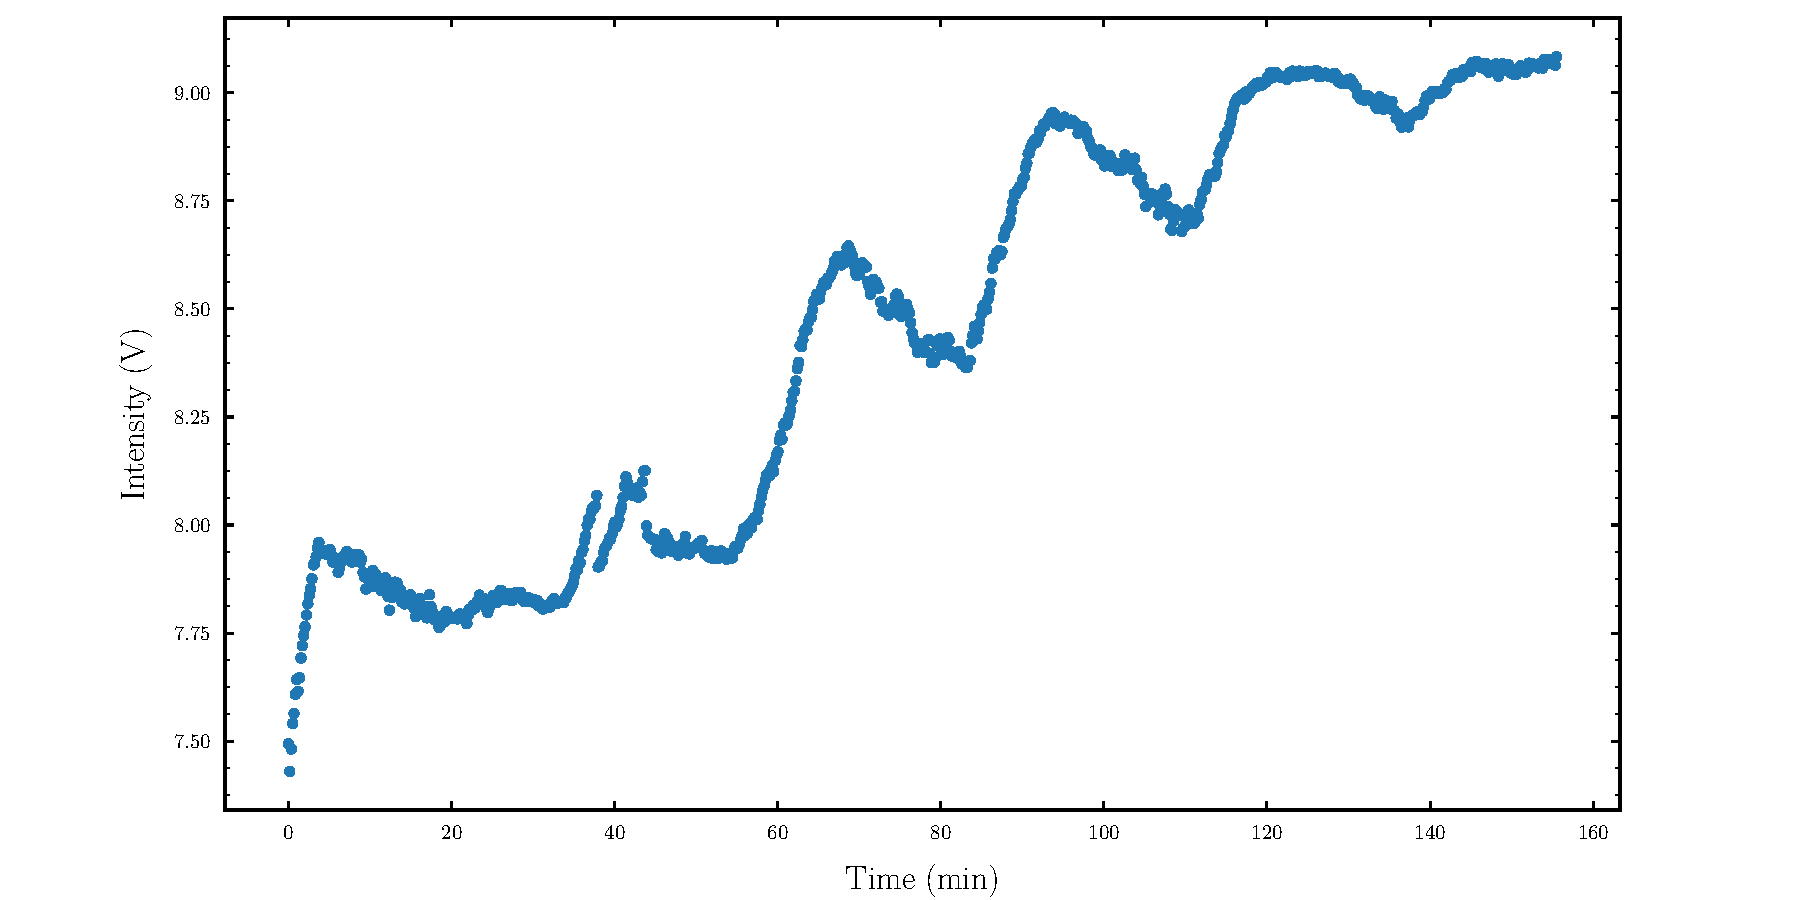
\includegraphics[width=\textwidth]
  {../figure/intensity/control/uncontrolled.pdf}
  \caption{Time evolution of the uncontrolled laser intensity.
  }\label{fig:intensity_uncontrolled}
\end{figure}
The setup used to record the intensity evolutions is disclosed in
\Cref{fig:intensity_control_setup}. It differs from the optical setup
described in \cref{ch:experimental_setup} by the absence of the \gls{aod}
and the relocation of Photodiode 2 at the end of the laser beam. The
photodiode gain of Photodiode 2 was lowered from \SI{70}{\decibel} to
\SI{50}{\decibel} because the lack of \gls{aod}s would otherwise cause the
photodiode to saturate.
\begin{figure}[htb]
  \centering
  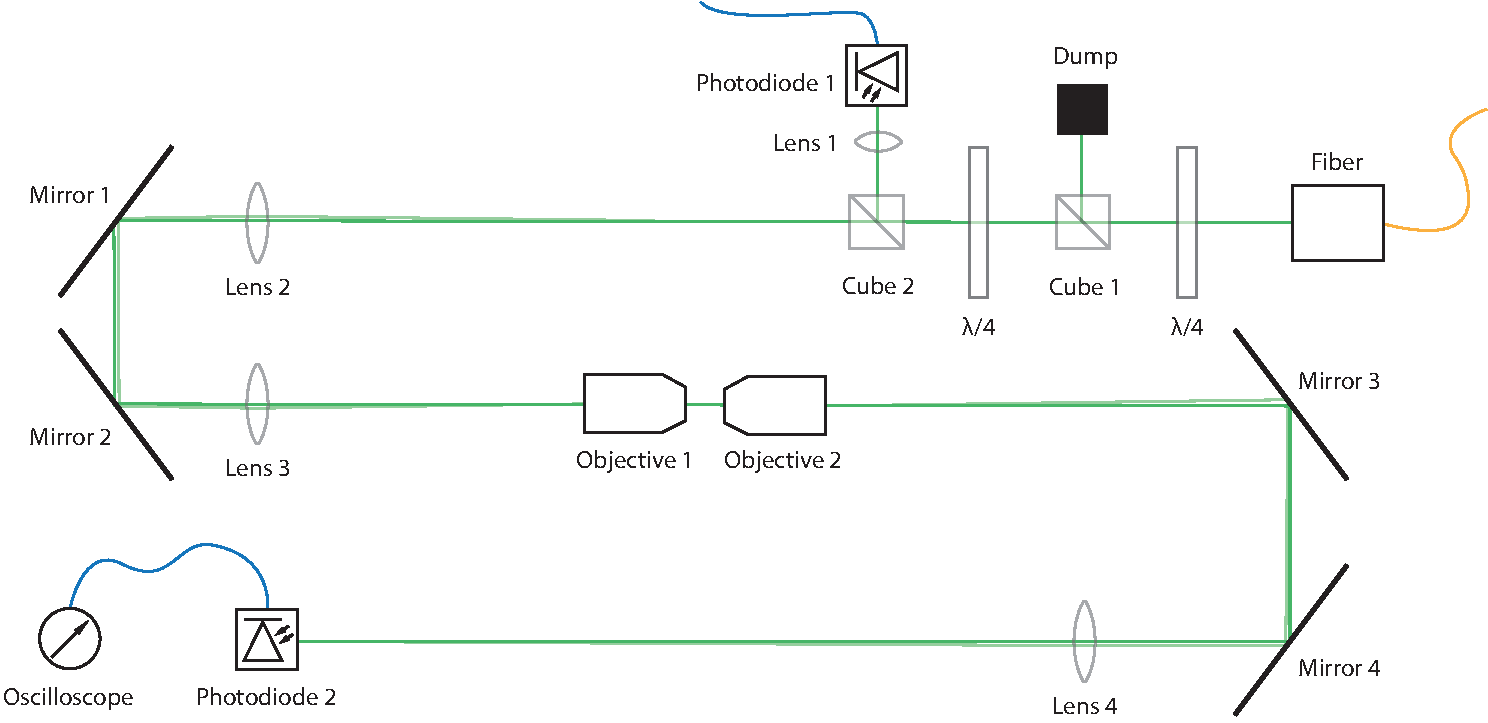
\includegraphics[width=.9\textwidth]{../media/setup/intensity-control.pdf}
  \caption{Optical setup and intensity detection. The beam hits Photodiode 2
    which is connected to the oscilloscope.
  }\label{fig:intensity_control_setup}
\end{figure}
In order to to estimate the error contribution due to imperfect intensity
regulation, we will conduct a short- and a long-term measurement of the
controlled intensity. Technically a typical intensity measurement takes about
a fraction of a millisecond, yet we can decide on different intervals between
the measurements in order to separate local from global trends like the ones
noted in the uncontrolled meausrement. \Cref{tab:intensity_control_times}
summarizes the different time scales for the conducted short- and long-term
measurement of the intensity control.
\begin{table}[htb]
  \centering
  \begin{tabular}{cccc}
    \toprule
    & Short & Long & Typical \\
    \midrule
    Interval &
    \SI{10}{\second} &
    \SI{120}{\second} &
    \SI{3}{\second} \\
    Duration &
    \SI{1}{\hour} &
    \SI{16}{\hour} &
    \SI{<2}{\hour} \\
    \bottomrule
  \end{tabular}
  \caption{Interval and duration times of the short- and long-term measurement
    as well as a typical sweep measurement.
  }\label{tab:intensity_control_times}
\end{table}
The voltage time series for both intensity control measurements are presented
in \Cref{fig:intensity_control}. The outlier at about 22:45 h was caused by
accidently interfering with the setup during measurement. Beside of that
incident the long-term intensity seems stable. On a smaller timescale we see
that the intensity evolution performs periodic oscillations.
\begin{table}[htb]
  \centering
  \begin{tabular}{lcccc}
    \toprule
    Measure & Uncontrolled & Long & Short & Typical \\
    \midrule
    Mean $\mu$ &
    \SI{8.45}{\volt} &
    \SI{6.79}{\volt} &
    \SI{6.79}{\volt} &
    \SI{1.95}{\volt} \\
    Minimum &
    \SI{7.43}{\volt} &
    \SI{4.88}{\volt} &
    \SI{6.77}{\volt} &
    \SI{0.00}{\volt} \\
    Maximum &
    \SI{6.82}{\volt} &
    \SI{6.86}{\volt} &
    \SI{6.82}{\volt} &
    \SI{9.08}{\volt} \\
    Standard Deviation $\sigma$ &
    \SI{0.49}{\volt} &
    \SI{0.09}{\volt} &
    \SI{0.01}{\volt} &
    \SI{0.54}{\volt} \\
    Relative Standard Deviation $\sigma/\mu$ &
    \SI{5.75}{\percent} &
    \SI{1.35}{\percent} &
    \SI{0.19}{\percent} &
    \SI{27.69}{\percent} \\
    \bottomrule
  \end{tabular}
  \caption{Descriptive statistics of uncontrolled and controlled short- and
    long-term intensity evolutions as well as a typical intensity measurement
    with \gls{aod}s for comparison.
  }\label{tab:intensity_control_statistics}
\end{table}
Overall we can confirm that the intensity control loop successfully holds the
intensity mean, though with small oscillations. In order to estimate the
relevance for these small oscillations of the controlled intensity for later
measurements, we selected an measurement of the intensity transmission
response of the \gls{aod} subject to constant frequency increments for
comparison. \Cref{tab:intensity_control_statistics} presents the statistics of
said intensity measurements.
\begin{figure}[htb]
  \centering
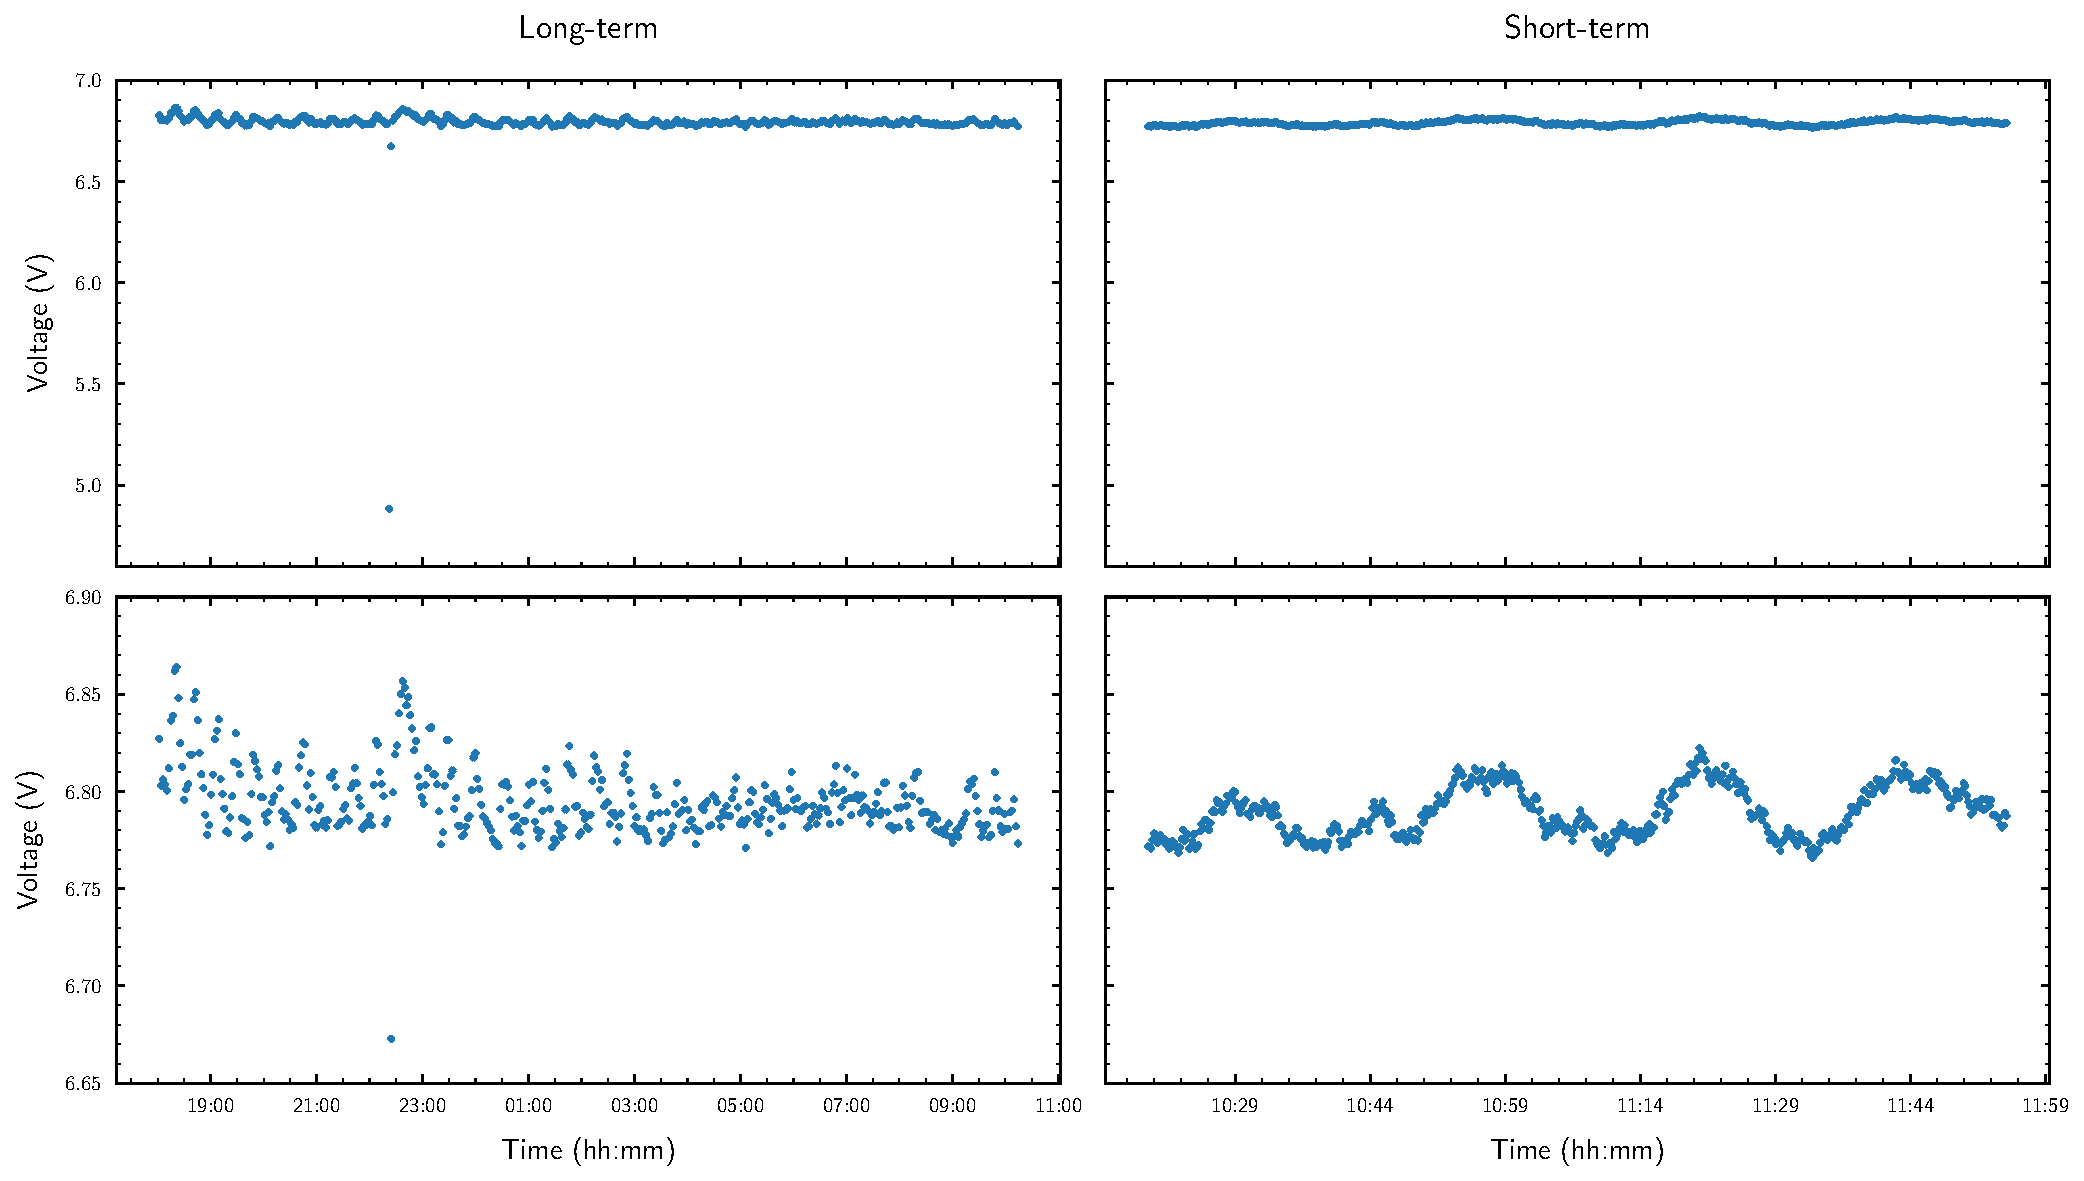
\includegraphics[width=\textwidth]{../figure/intensity/control/long-short.pdf}
  \caption{Long- and short-term measurement of the controlled intensity at
    different voltage scales.
  }\label{fig:intensity_control}
\end{figure}
We should note that not all of the statistical measurements are directly
comparable because of the \SI{20}{\decibel} higher photodiode gain used in
the typical measurement with \gls{aod}s. Nevertheless we can directly compare
the uncontrolled and the controlled short- and long-term measurements
directly. As we divide by the mean $\mu$, the relative standard deviation
$\sigma/\mu$ is a scale invariant statistical measure and thereby comparable
through measurements conducted with different photodiode gain setting.
Comparing the relative standard deviation yields that the intensity drifts
are small on a short time scale compared to intensity variations in a typcial
measurement. In contrast the uncontrolled intensity --- also conducted on
a short-term time scale --- contributes a significant error. In order to
compare the intensity deviations further we calculate the \gls{rmd} via
\begin{equation}
  I_\text{rmd}
  =
  \frac{I-\overline{I}}{\overline{I}}
  \label{eq:relative_mean_deviation}
\end{equation}
where $\overline{I}$ denotes the intensity mean. In
\Cref{fig:intensity_control_rmd} the \gls{rmd} of the controlled and
uncontrolled as the controlled measurements are presented as boxplots.
\begin{figure}[htb]
  \centering
  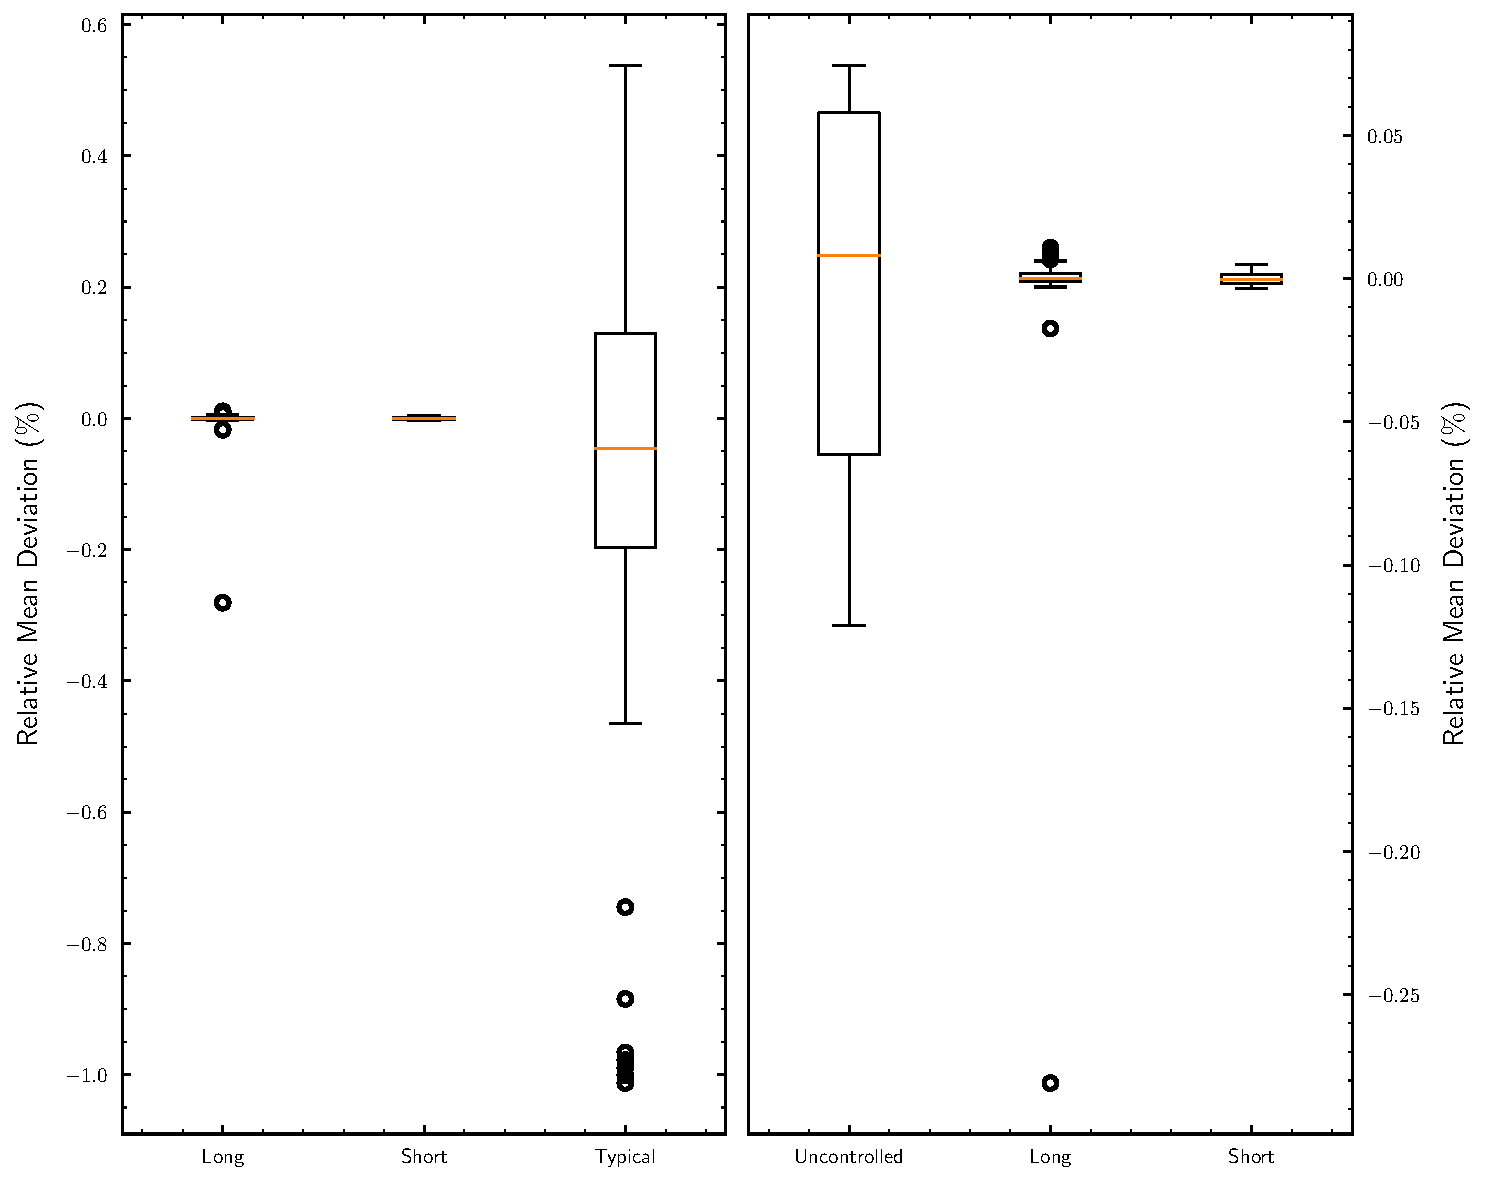
\includegraphics[width=\textwidth]
{../figure/intensity/control/relative-mean-deviation.pdf}
  \caption{Relative mean deviation of uncontrolled and controlled long- and
    short-term measurement as well as typical controlled intensity measurement.
  }\label{fig:intensity_control_rmd}
\end{figure}
Boxplots are heavily based on the concept of \gls{iqr}. The \gls{iqr} is a
scale invariant measure of statistical dispersion and is defined as the
inverse of the \gls{cdf}. The start and end of the boxes inside a boxplot
denote the lower (first) quantile $Q_1$ and the upper (third) quantile $Q_3$
of the \gls{iqr}. Expressed through the \gls{cdf} these read
\begin{align}
  Q_1=\text{CDF}^{-1}{\left(\frac{1}{4}\right)} &&
  Q_3=\text{CDF}^{-1}{\left(\frac{3}{4}\right)}.
\end{align}
Alternatively one can define $Q_1$ as the median of the $n$ smallest entries
and $Q_3$ as the median of the $n$ largest entries where the total dataset
consists out of $2n$ entries for the even and $2n+1$ entries for the odd case.
The whiskers below and atop of the boxes are at $Q_1\pm1.5IQR$. Values outside
this range are usually considered outliers and marked as circles. The median
is denoted with an orange line. The left boxplot confirms that the
oscillations of the controlled intensity are negligible for typical intensity
measurements. Further the right boxplot confirms that the intensity control
oscillations cover a much smaller range as the uncontrolled oscillations.

\section{Beam profile}

Perpendicular to the error introduced by the imperfect intensity control,
errors can originate from unideal optical alignment. One way to assess the
quality of our alignment is to evaluate the spatial profile of the laser beam
as registered with the \gls{ccd} camera.
\begin{figure}[htb]
  \centering
  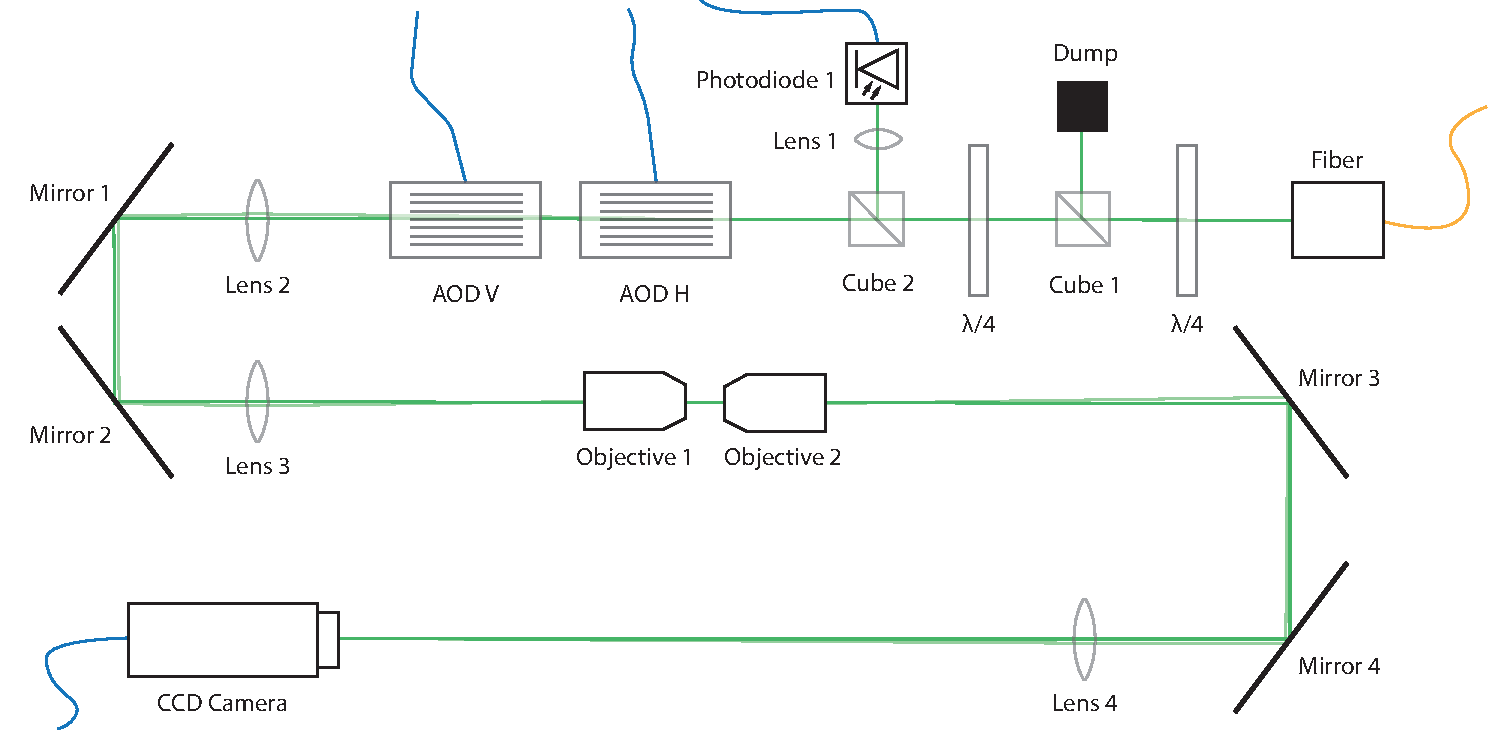
\includegraphics[width=\textwidth]{../media/setup/intensity-profile.pdf}
  \caption{The beam is focused onto the \gls{ccd} sensor of the camera.
  }\label{fig:intensity_profile_setup}
\end{figure}
In \Cref{fig:intensity_profile_setup} we present the setup used to measure
the spatial beam profile. In comparison to the previous setup we replaced
Photodiode 2 with a \gls{ccd} camera. The \gls{aod}s are configured at a
center frequency of \SI{100}{\mega\hertz}. The distance between Lens 4 and
the \gls{ccd} sensor is chosen such that the laser beam is focused onto the
\gls{ccd} sensor of the camera.
\begin{figure}[htb]
  \centering
  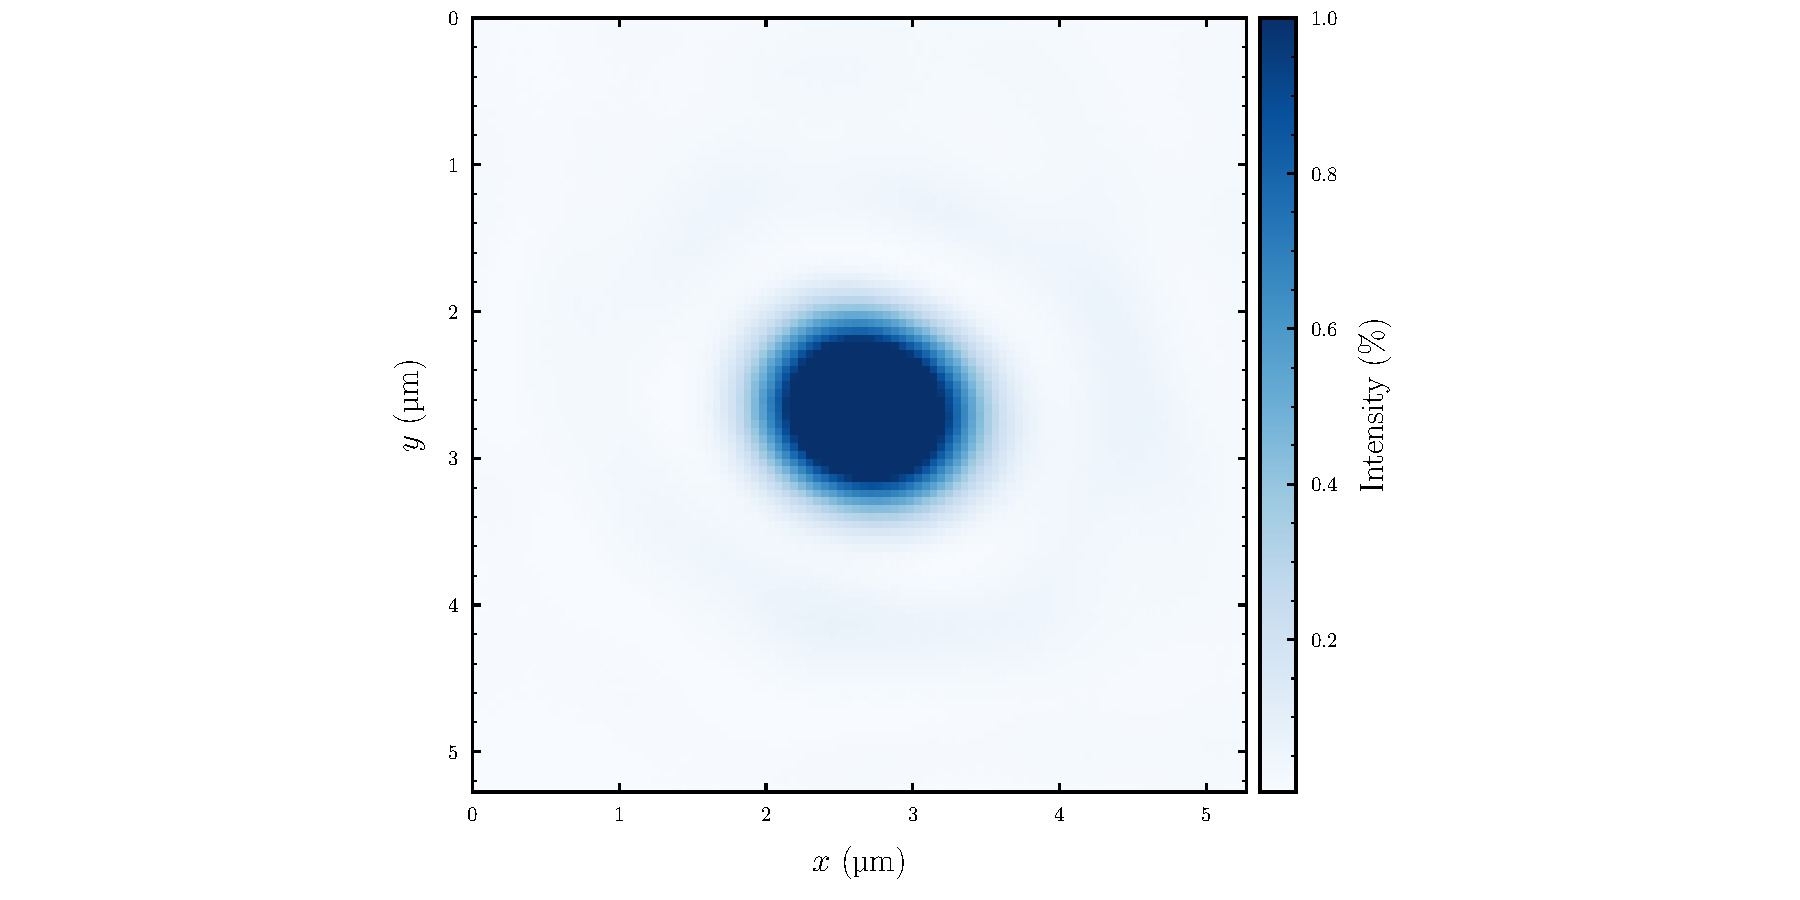
\includegraphics[width=.6\textwidth]
  {../figure/intensity/profile/image.pdf}
  \caption{Image of the focused laser beam measured with the \gls{ccd} camera.
  }\label{fig:intensity_spatial_image}
\end{figure}
\Cref{fig:intensity_spatial_image} shows an enlarged image patch of the
complete image capture taken with the \gls{ccd} camera. We can see a strong
illuminated circular spot in the center of the image with an area of about
\SI{2.5}{\milli\meter}. The intensity inside the spot seems homogeneous,
however this is caused by a saturation of the pixels in this area. We could
reduce the intensity or apply an optical filter to the camera to resolve the
intensity gradient inside the spot, but only at the cost of the intensity
distribution around the spot. Around the circular spot we can see a
diffraction ring. The diffraction ring is well described
in~\cite{Hertlein2017} and originates from the finite aperture of the
objectives.
\begin{figure}[htb]
  \centering
  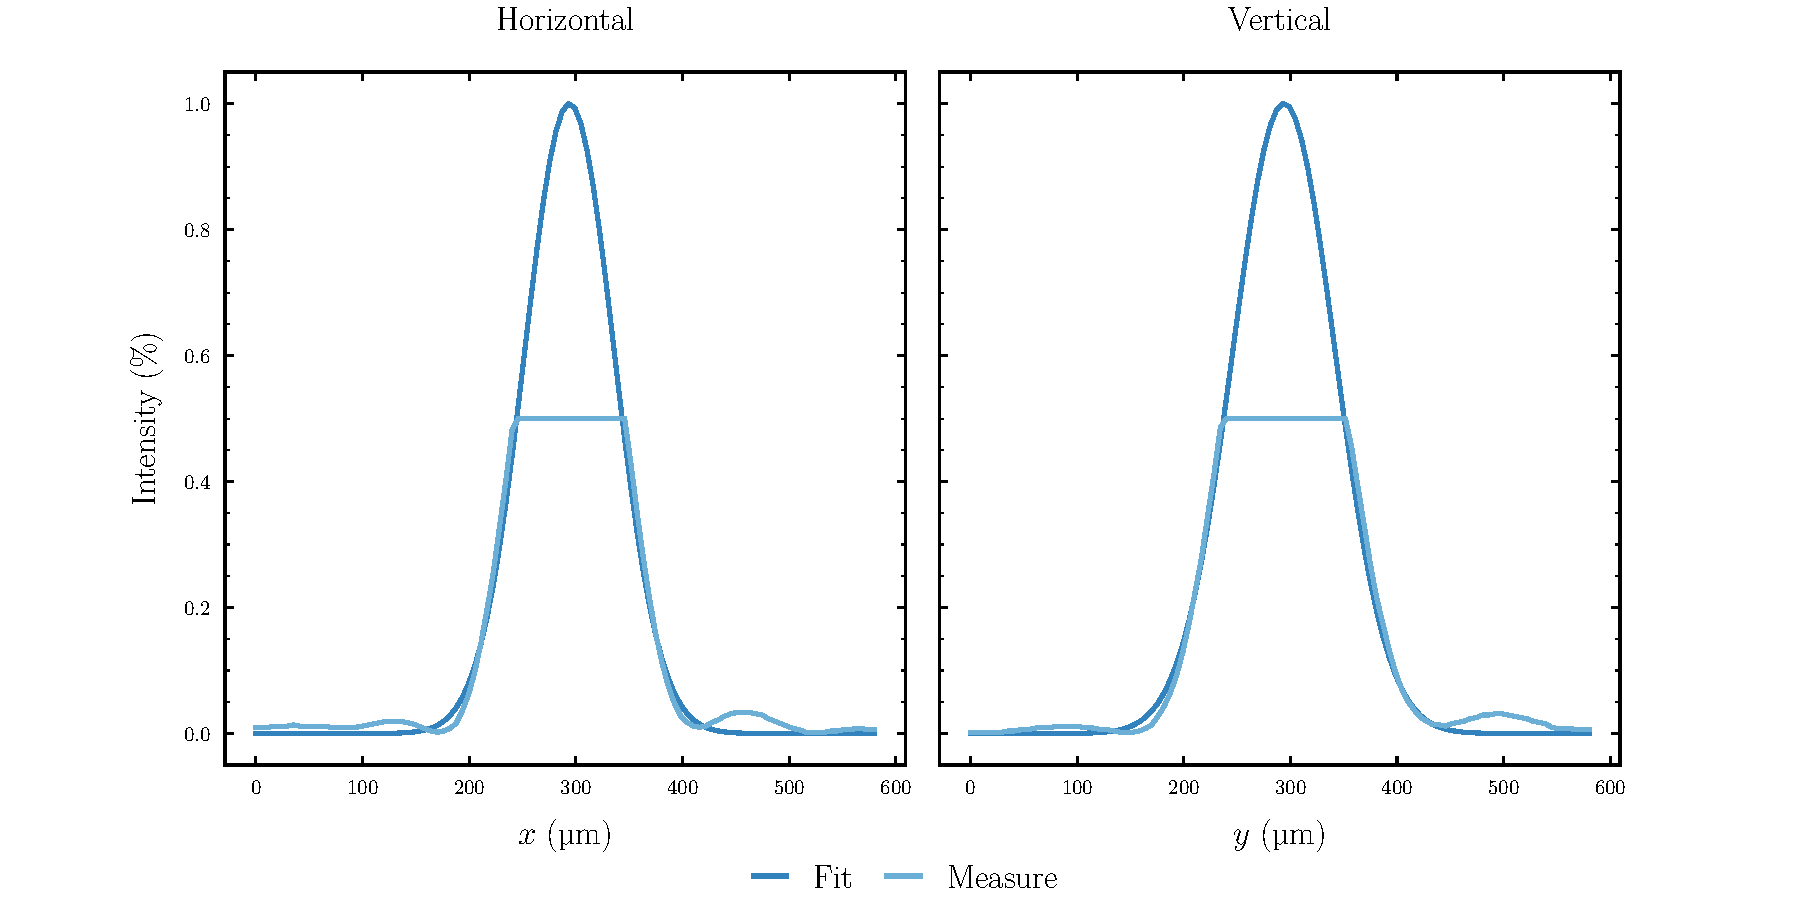
\includegraphics[width=.9\textwidth]{../figure/intensity/profile/profile.pdf}
  \caption{One dimensional perpendicular cut of the two dimensional intensity
    distribution from the two dimensional beam profile in
    \Cref{fig:intensity_spatial_image} with fitted gaussian curve.
  }\label{fig:intensity_spatial_profile}
\end{figure}
For better comparison of the radial symmetry we performed two perpendicular
cuts and visualized the one dimensional spatial beam distribution in
\Cref{fig:intensity_spatial_profile}.
In \Cref{fig:intensity_spatial_profile} we can clearly observe the effects of
saturation around the center and how we would expect the intensity to be
if we could experimentally resolve it in the Gaussian fit. In contrast to the
ideal Gaussian profile we again observe contributions to the Airy disc around
the otherwise Gaussian profile causes by the finite aperture. Further we can
now clearly observe assymmetry from the intensity contributions around the
Gaussian which means that our alignment is not perfect.

We can confirm the results reported in~\cite{Hertlein2017} that the spatial
beam profile equals a two dimensional Gaussian combined with a Airy disks
caused from the finite aperture of the objectives. Further we observe
slight assymmetries in the diffraction ring suggesting inperfect alignment.
Though asymetries in the spatial beam profile are present, we do not see any
further complications as the intensity measurements with the photodiode will
cover the complete beam profile.

\section{Difference between individual acousto-optic deflectors}

Our optical setup uses a single two dimensional \gls{aod} that comprises two
\gls{aod} elements perpendicular to each other. At first we want to examine the
behaviour of the individual \gls{aod} elements to each other. In particular we
are interested if and how the elements differ.
\begin{figure}[htb]
  \centering
  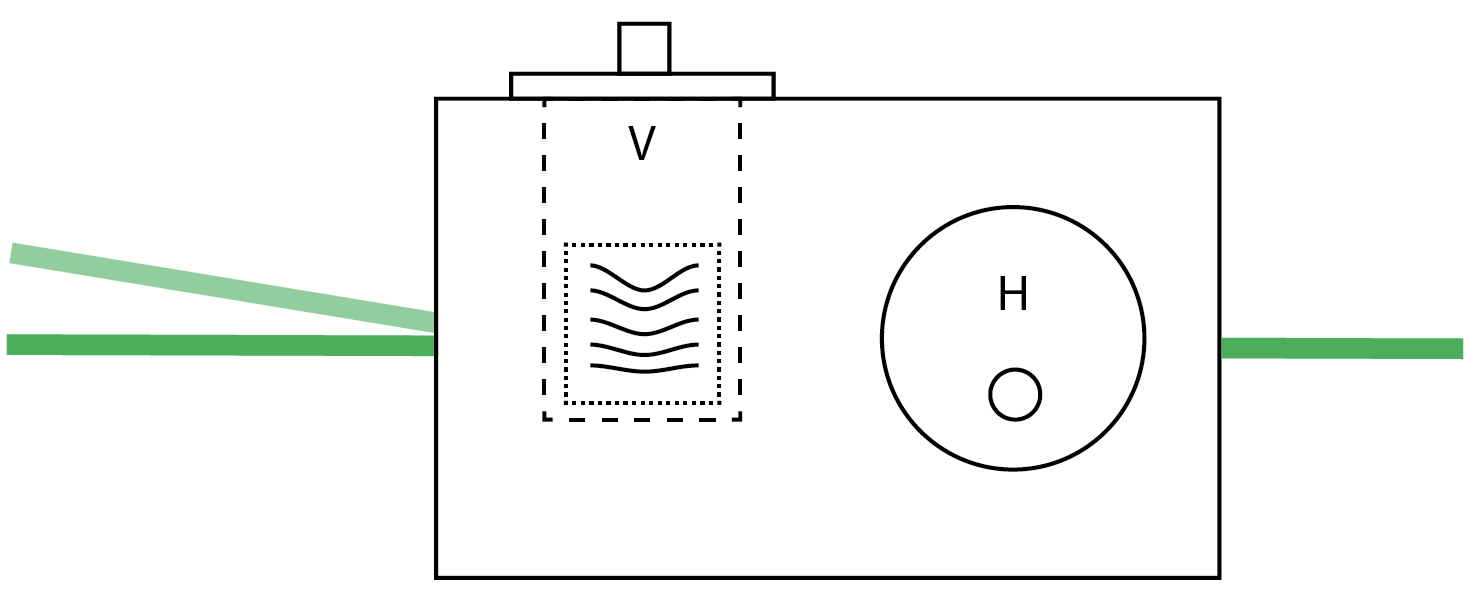
\includegraphics[width=\textwidth]{../media/setup/aod-socket.png}
  \caption{Drawing of the used 2D \gls{aod}.
  }\label{fig:aod_socket}
\end{figure}
A schematic drawing of the \gls{aod} is depicted in \Cref{fig:aod_socket}. We
see the two \gls{aod} elements in the respective horizontal and vertical slot.
The internals of the vertical \gls{aod} (left-hand side) are illustrated. The
element itself spans through the casing (dashed line) while the acousto-optic
crystal (dotted line) is glued onto the element. The laser beam (green) passes
through the acousto-optic crystal. In the following we will refer to the
horizontal \gls{aod} element as the \gls{aod} element anticipated for the
horizontal slot and accordingly to the vertical \gls{aod} element as the
\gls{aod} element intended for the vertical \gls{aod} socket.

\subsection{Individual acousto-optic deflectors}

For the following experiment we will only leave one \gls{aod} element mounted
in the casing depicted in \Cref{fig:aod_socket}. The other slot will be empty.
Then we will exchange socket positions for each respective \gls{aod} element
and measure the beam intensity subject to the linear frequency sweep from
\SI{80}{\mega\hertz} to \SI{120}{\mega\hertz} over a duration of
\SI{260}{\milli\second} and the configured \gls{dds} amplitude. As \gls{rf}
signal source the amplifier and \gls{dds} combination intended for the
horizontal \gls{aod} element was used to avoid influences of the amplification
offset between the two amplifiers.
\begin{figure}[htb]
  \centering
  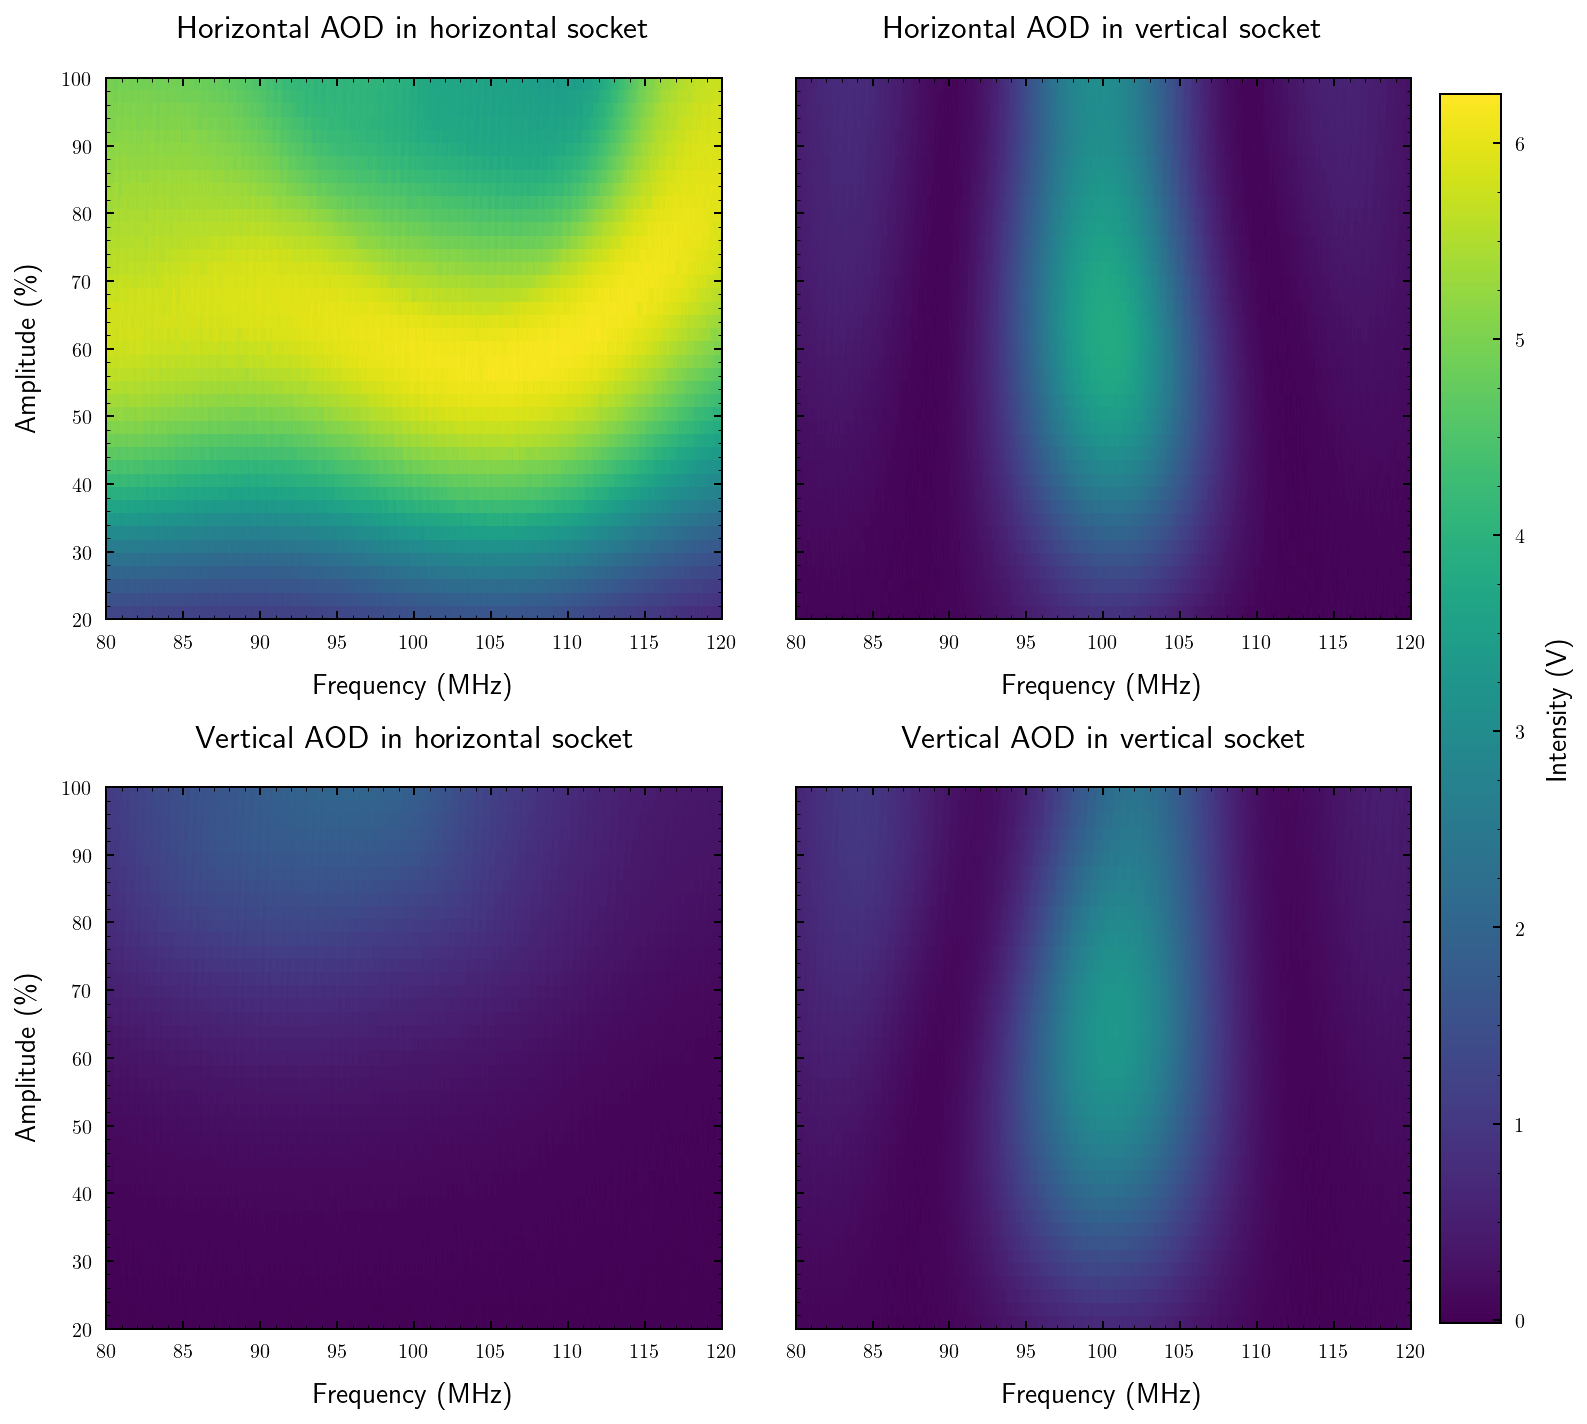
\includegraphics[width=\textwidth]
  {../figure/intensity/distribution/unpaired-amplitude.png}
  \caption{Intensity distribution over linear frequency sweep at different
    configured \gls{dds} amplitudes for different individual \gls{aod}
    configurations.
  }\label{fig:intensity_distribution_unpaired}
\end{figure}
The results for the four configurations (horizontal element in horizontal
slot, horizontal element in vertical slot, vertical element in horizontal
slot and vertical element in vertical slot) are visualized as heatmaps in
\Cref{fig:intensity_distribution_unpaired}. The color values are normalized in
between the different heatmaps and can be related to the measured voltage from
the photodiode via the colorbar on the right-hand side. Oddly enough we
observe that both \gls{aod}s differ strongly in their respective intensity
transmission behaviour depending on their slot position. Furthermore we
observe that the intensity transmission is much higher in the case of the
horizontal \gls{aod} element mounted to the intended horizontal slot compared
to all other configurations. In addition we can see that the intensity map
measured with the horizontal \gls{aod} displays a jump. The highest intensity
transmission is obtained for relative amplitudes configured between
\SI{60}{\percent} and \SI{90}{\percent} with large dependence on the
frequency. Another interesting observation is that the intensity transmission
seems very similar for the horizontal element in the vertical slot and the
vertical element in the vertical slot whose map also seems more symmetric with
respect to the frequency axis. In fact for these configurations the amplitude
dependence seems to be essentially independent of the frequency dependence.
We assume that the individual elements are designed for different
polarisation angles. In order to prove this hypothesis we added a tunable
$\lambda/2$ retarder plate after Cube 2. Tuning the $\lambda/2$ retarder
before Cube 2 would change the intensity fraction that gets redirected into
the beam dump as Cube 2 is a beam splitter sensible to polarisation.
\begin{figure}[htb]
  \centering
  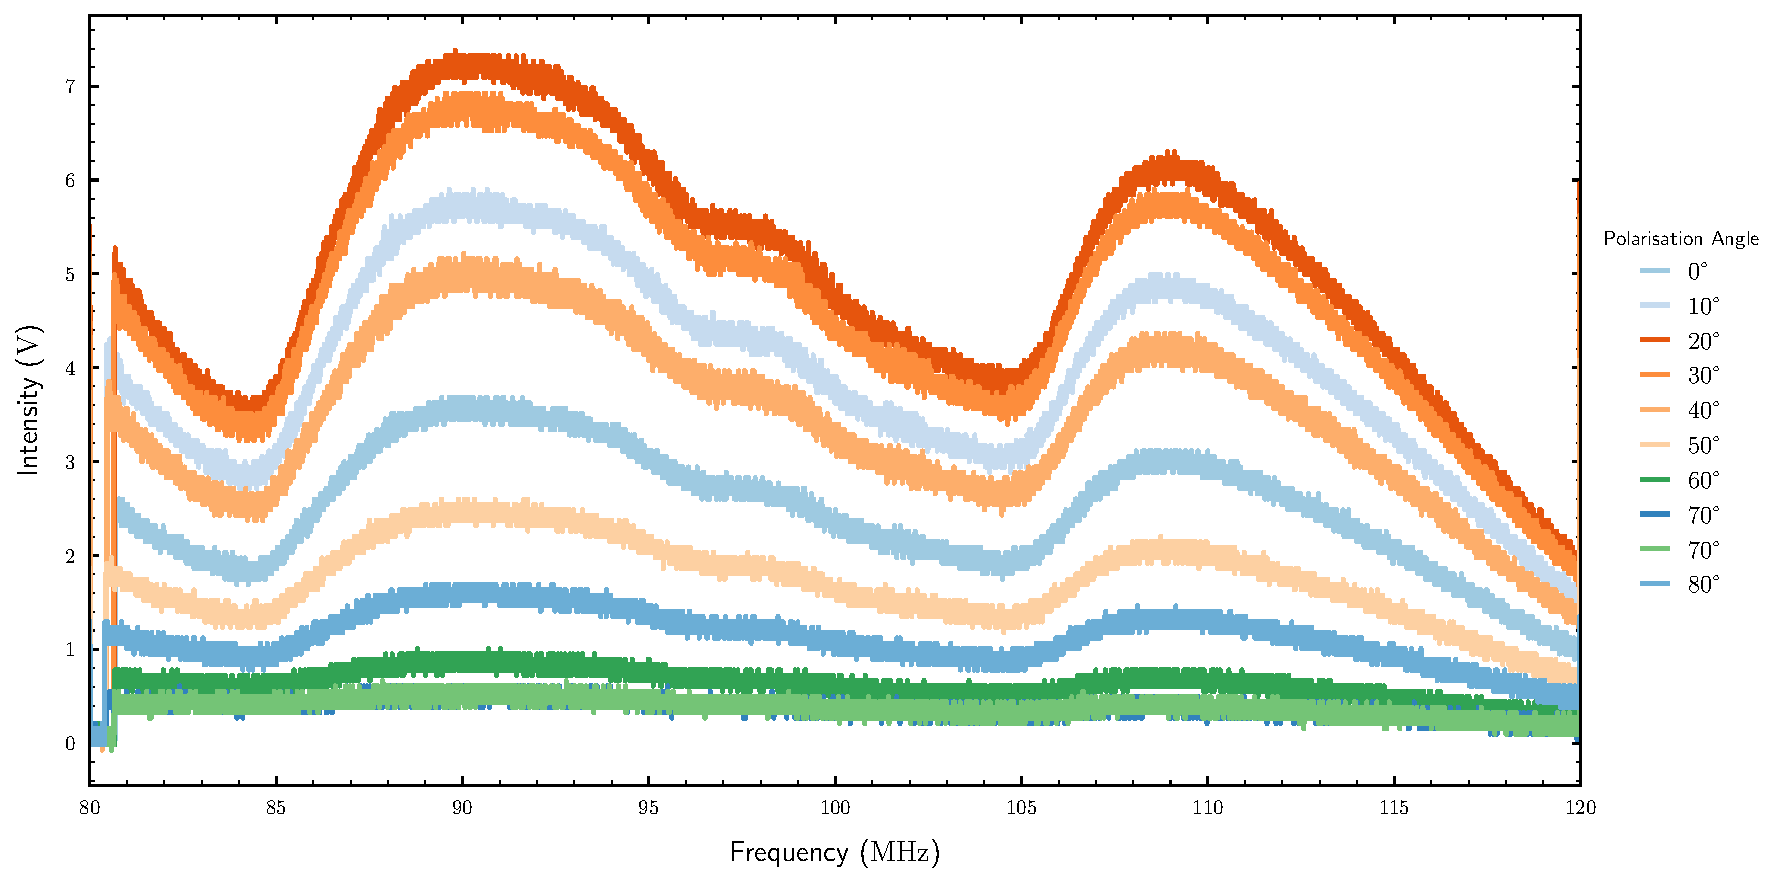
\includegraphics[width=\textwidth]
  {../figure/intensity/distribution/polarisation-horizontal.pdf}
  \caption{Intensity transmission of the \gls{h} \gls{aod} in the \gls{h} slot
    at maximum output amplitude for different polarisation angles.
  }\label{fig:intensity_polarisation_h}
\end{figure}
In \Cref{fig:intensity_polarisation_h} the intensity transmission of the
\gls{h} \gls{aod} in the \gls{h} slot at maximum output amplitude is presented
for different polarisation angles. The polarisation angles are the remainders
of the angles read of from the retarder plate mount divided by \ang{90}. The
reason behind this step is that a rotation of a retarder plate by $\phi$
effectively changes the polarisation angle by $2\phi$. Further the
polarisation domain is limited to $\left[0,\ang{90}\right]$.
\begin{figure}[htb]
  \centering
  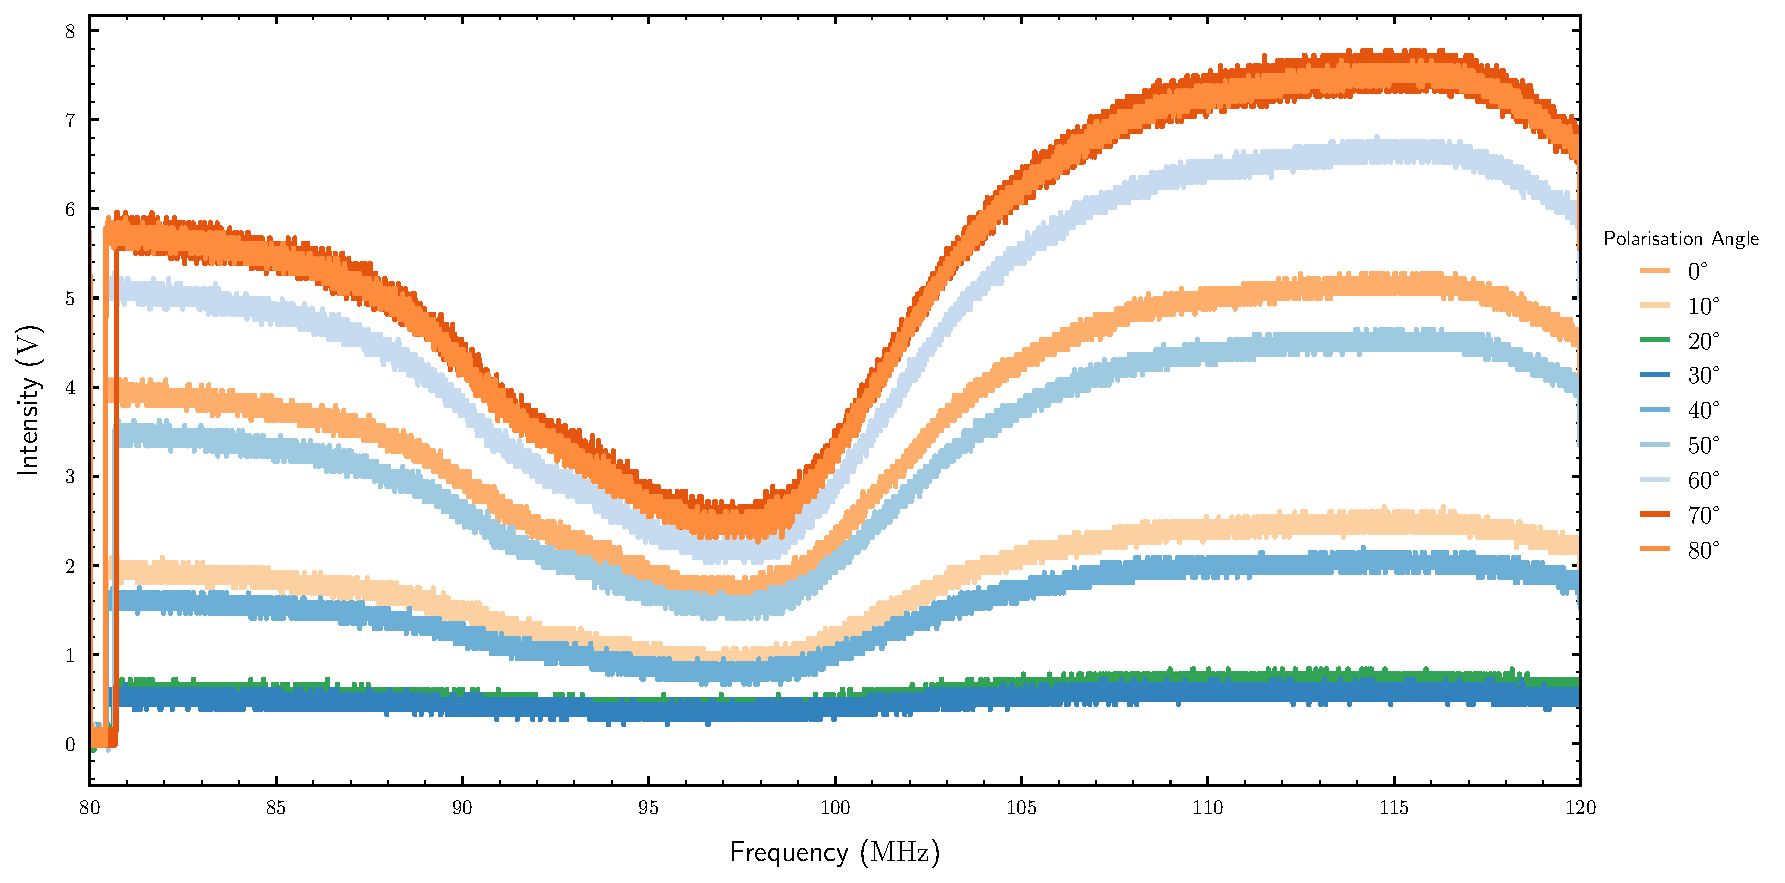
\includegraphics[width=\textwidth]
  {../figure/intensity/distribution/polarisation-vertical.pdf}
  \caption{Intensity transmission of the \gls{v} \gls{aod} in the \gls{v} slot
    at maximum output amplitude for different polarisation angles.
  }\label{fig:intensity_polarisation_v}
\end{figure}
We note the maximum intensity transmission of the \gls{h} \gls{aod} at
\ang{20} and the minimum intensity transmission at around \ang{70}. The
difference between the polarisation angle at minimum and maximum intensity
is about \ang{50} which is close to \ang{45} that would suggest that
intensity minimum and maximum are located at the respective perpendicular
polarisation axis. In \Cref{fig:intensity_polarisation_v} the intensity
transmission subject to the polarisation angle of the \gls{v} \gls{aod} in
the \gls{v} slot is shown. We again observe a difference of about \ang{45}
between the polarisation angles at maximum and minimum intensity transmission.
\begin{figure}[htb]
  \centering
  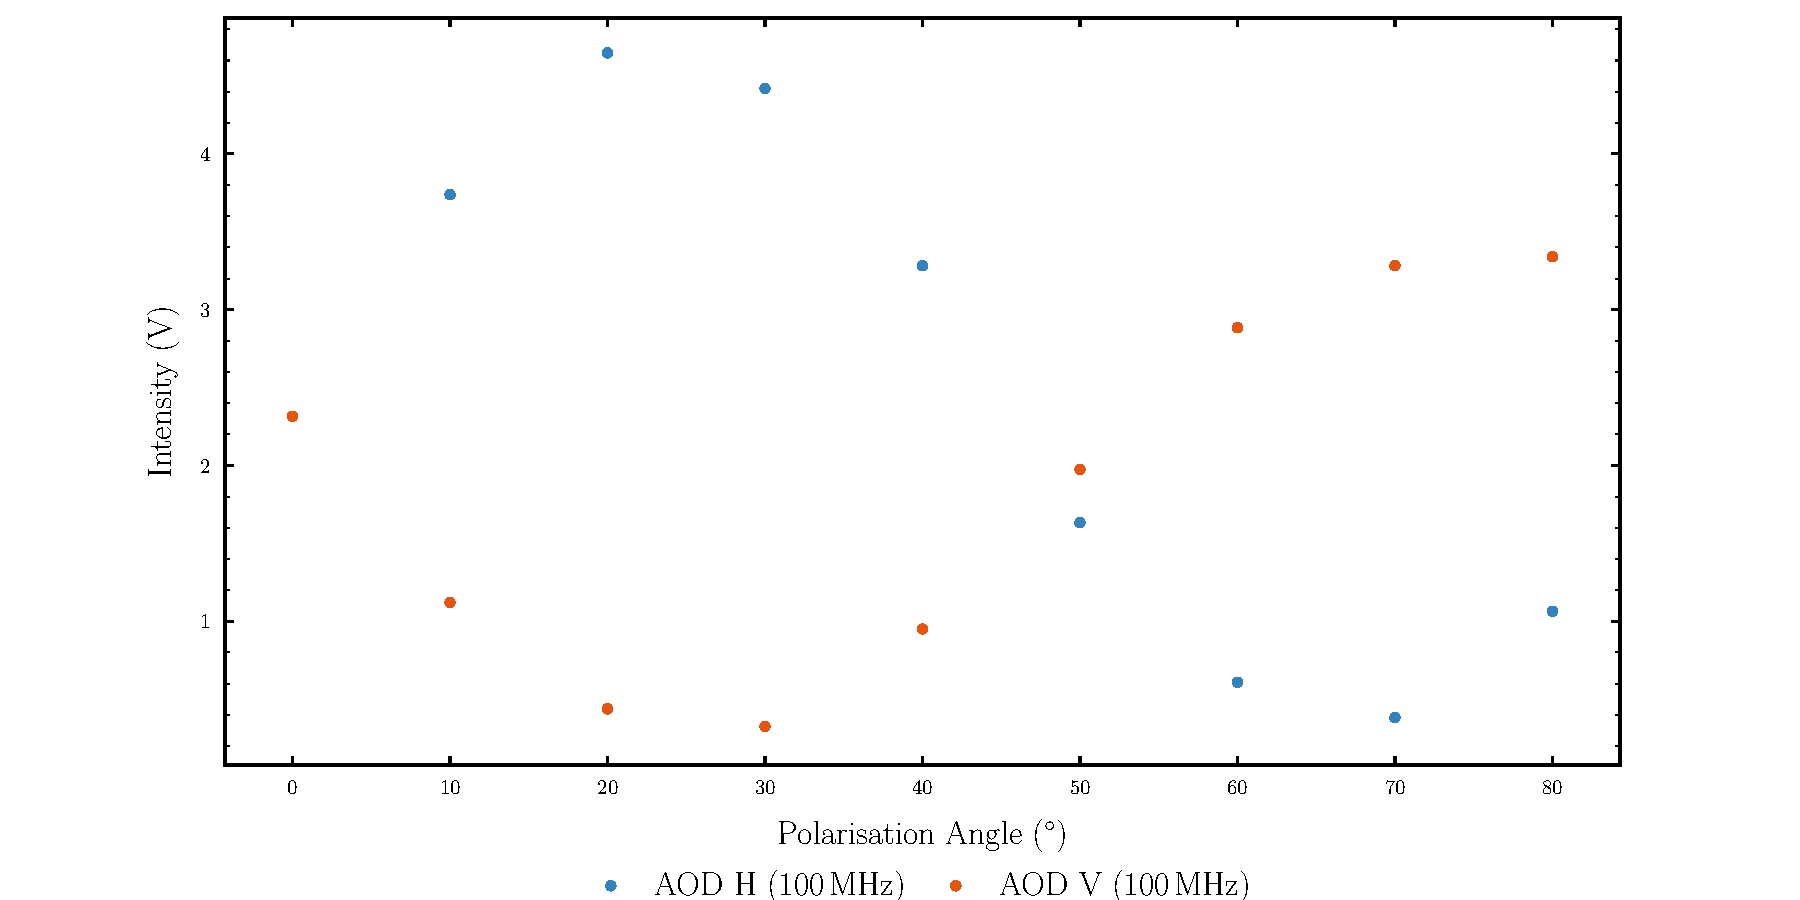
\includegraphics[width=\textwidth]
  {../figure/intensity/distribution/polarisation.pdf}
  \caption{Intensity transmission of the \gls{h} and \gls{v} \gls{aod} at
    \SI{100}{\mega\hertz} and maximum output amplitude for different
    polarisation angles.
  }\label{fig:intensity_polarisation}
\end{figure}
Finally we want to compare the polarisation angles between the individual
\gls{aod}s. Therefore we extracted the intensity transmission at
\SI{100}{\mega\hertz} frequency for both \gls{aod} measurements and plotted
them against the polarisation angle in \Cref{fig:intensity_polarisation}. We
observe a sinusoidal shaped intensity response of the polarisation angle
for the \gls{h} and \gls{v} \gls{aod} which seem out of phase by nearly
\ang{90}.

The 2D \gls{aod} casing allows to rotate the individual \gls{aod} elements. So
far we choose the rotation angle of the \gls{aod} elements that maximizes the
intensity transmission at the center frequency. What would we obtain if we
tilted the rotation angle a bit to the left and to the right?
\begin{figure}[htb]
  \centering
  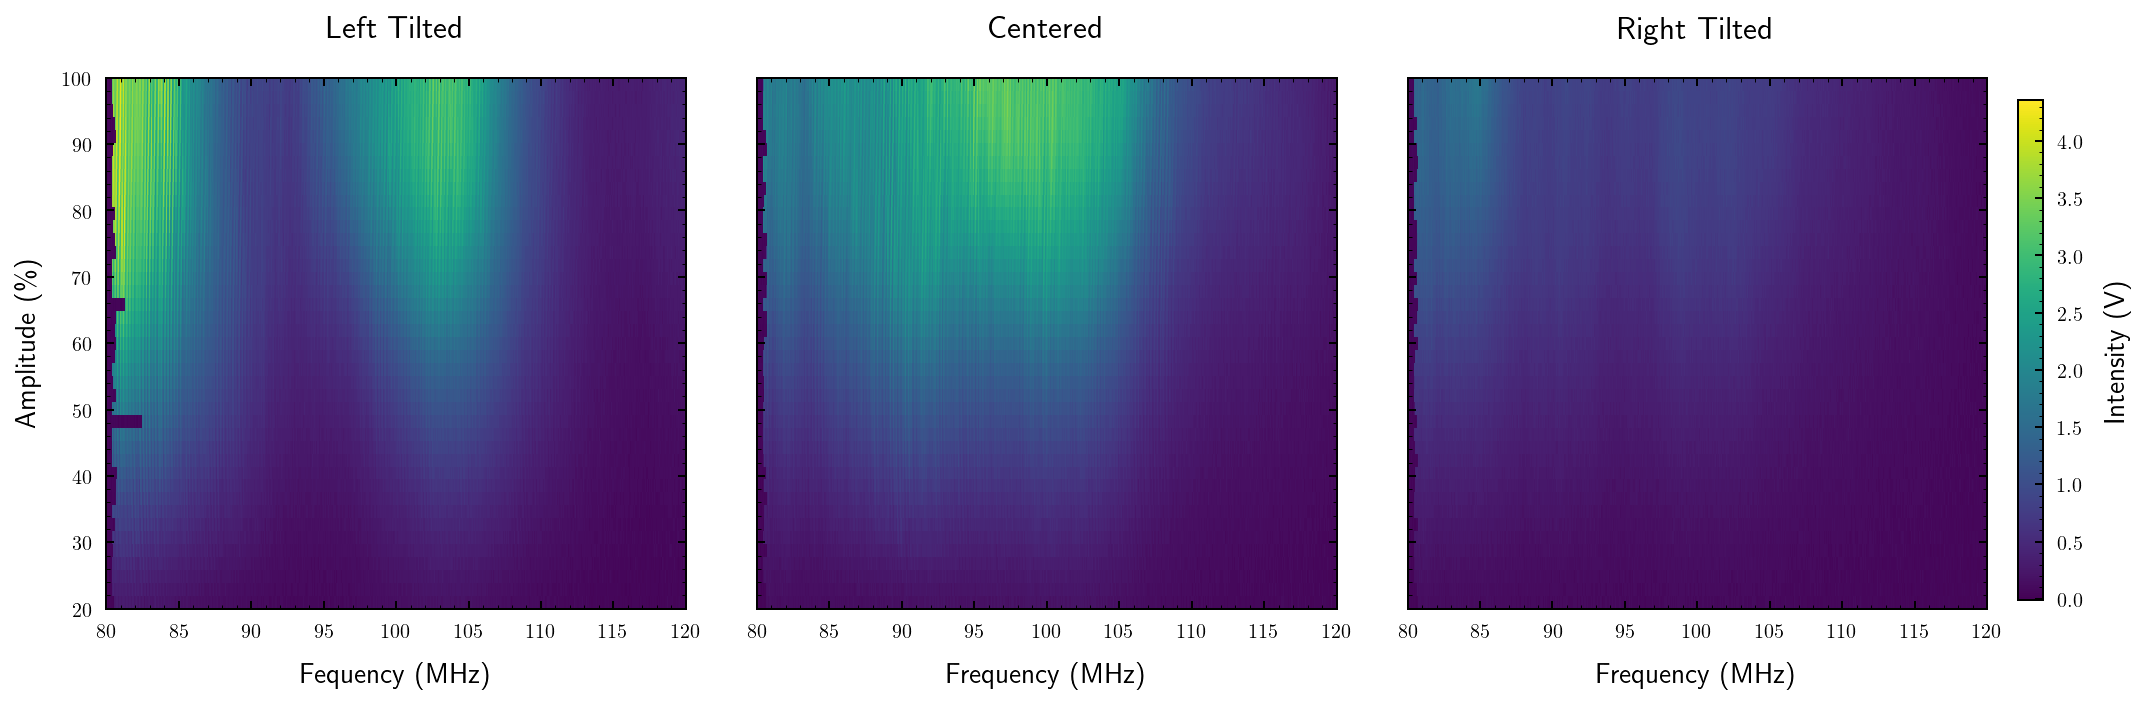
\includegraphics[width=\textwidth]
  {../figure/intensity/distribution/unpaired-tilted.png}
  \caption{Intensity distribution at different amplitudes for tilted
    individual \gls{aod}. We observe that the intensity decreases if the
    incident angle deviates from \ang{90}.
  }\label{fig:intensity_distribution_tilted}
\end{figure}
In \Cref{fig:intensity_distribution_tilted} we find the answer to this
question. We observe changes in shape and overall intensity with respect
to the incident angle. We should note that small changes in the incident
angle cause already large deflections of the beam, thus it is not guaranteed
that the left and right measurements are free from aperture effects.
Nevertheless we can record that the incident beam angle is an important
parameter in the intensity transmission of the \gls{aod}s. In particular we
need to consider the incident beam angle for the 2D \gls{aod} configuration.
It may make sense to change the setup to a configuration consisting of two
1D \gls{aod} with a telescope in between.

\subsection{Paired acousto-optic deflectors}

The \gls{aod} elements differ significantly in their intensity transmission
in between and with respect to their position. We find the horizontal element
in the anticipated horizontal position to have a significantly higher
transmission then any other configuration. Therefore we presume that the
\gls{aod} elements have a very high polarization dependency and are concerted
to eachother. We may find more evidence for this hypothesis by mounting both
\gls{aod} elements in their intended and exchanged slots.
\begin{figure}[htb]
  \centering
  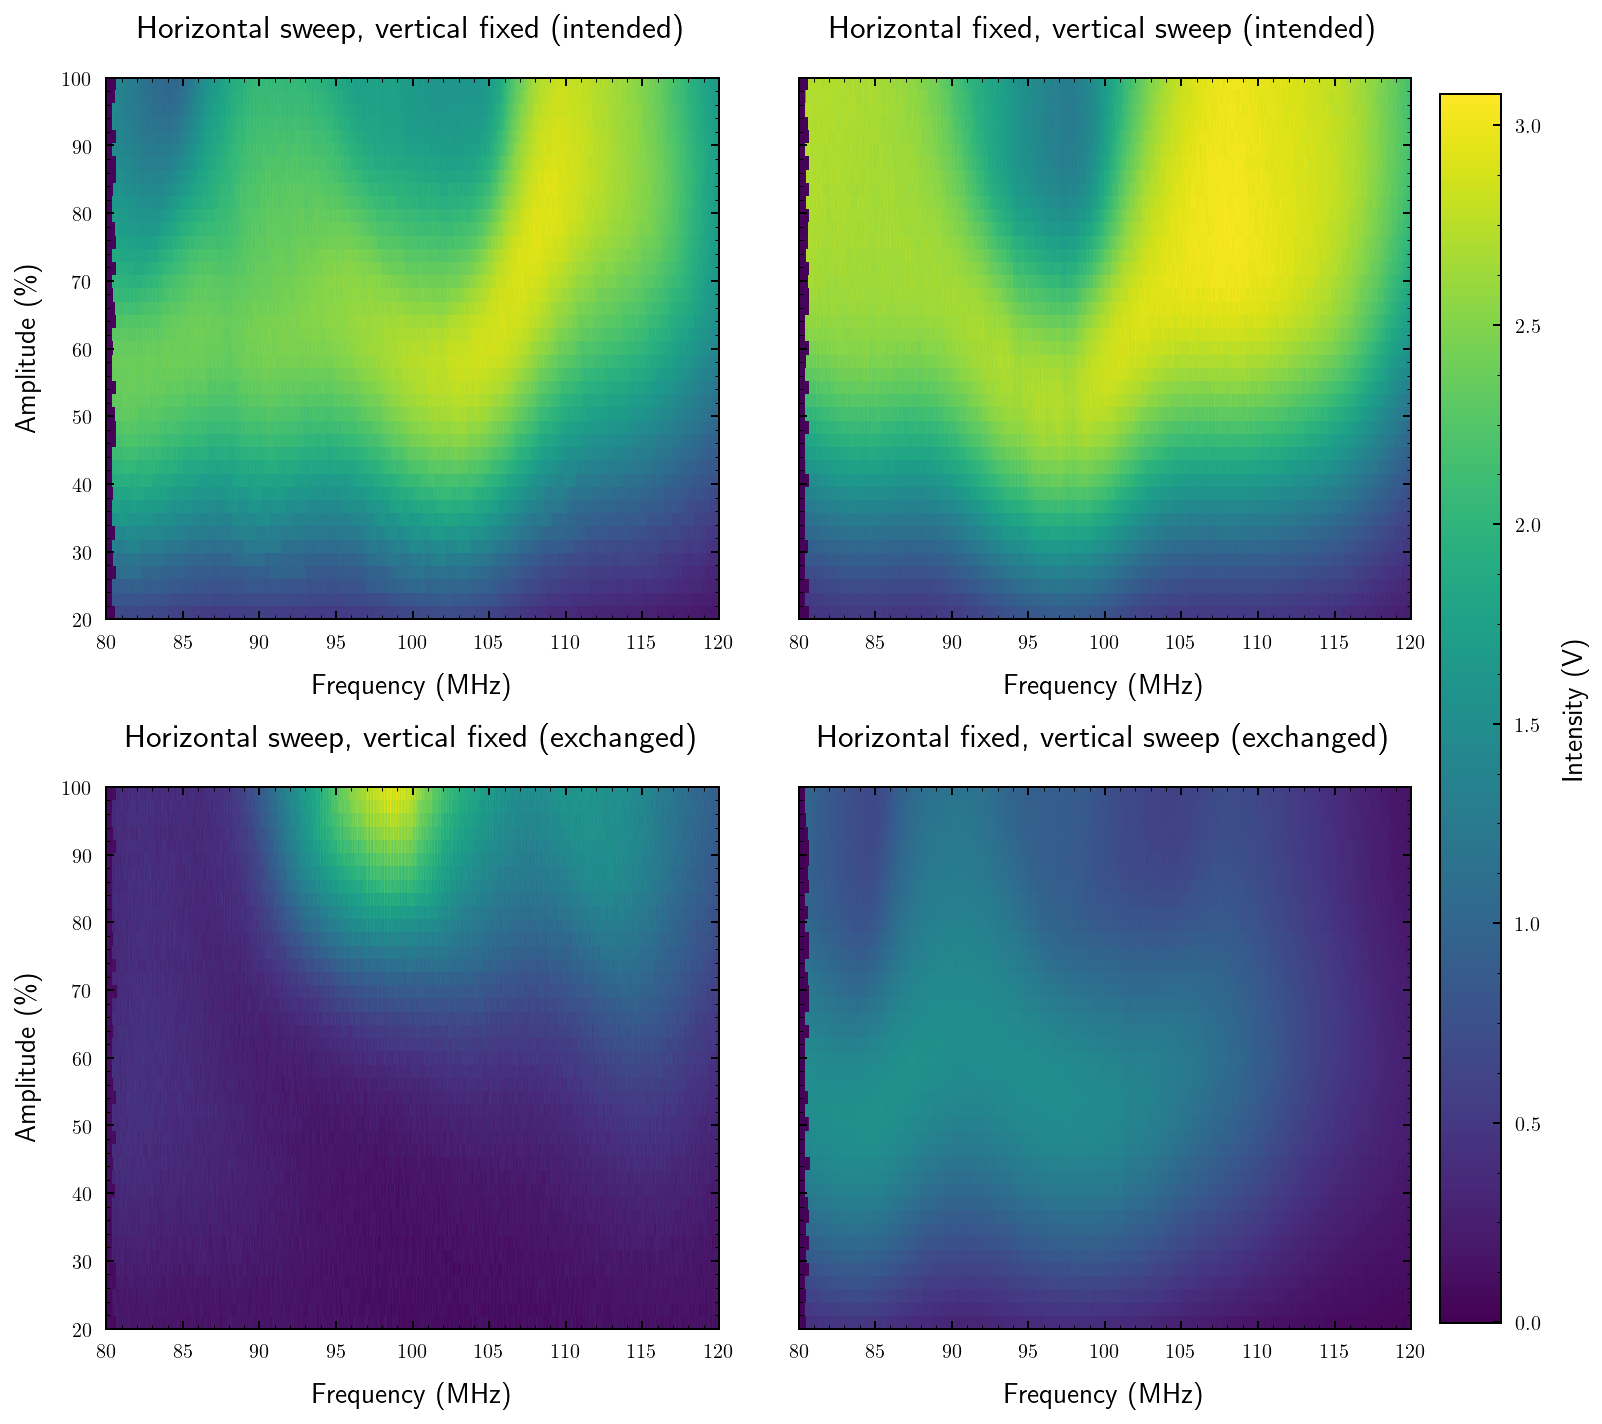
\includegraphics[width=\textwidth]
  {../figure/intensity/distribution/paired-amplitude.png}
  \caption{Intensity distribution over linear frequency sweep at different
  configured \gls{dds} amplitudes for different individual \gls{aod}
  configurations.
  }\label{fig:intensity_distribution_paired}
\end{figure}
In \Cref{fig:intensity_distribution_paired} the measured voltage of the
second photodiode are visualized in a two-dimensional heatmap. The horizontal
axis represents the frequency of the \gls{rf} signal applied to the \gls{aod}
elements whereas the vertical axis the configured \gls{dds} relative
amplitude. In the first row the elements where in their intended slots whereas
we exchanged them for the second row. In the first column the frequency
sweep was applied such that the beam moves along the horizontal axis while
in the second column the frequency sweep was applied to the element that
causes beam movement in the vertical direction.

We see that for the exchanged positions the transmission is reduced and
asymmetric with respect to the sweep direction whereas the elements in their
intended position perform better in every aspect. We therefore conclude that
the \gls{aod} are cut in a intended way to account among others for
polarization effects and it is advised to operate them in their anticipated
slot as we will do for all following experiments.

\section{2D intensity distribution}

In the previous section we sorted out the influence of the \gls{aod} element
position and acknowledged that \gls{aod}s differ significant in their
optical properties. In the present section we now want to explore the
intensity transmission for a two dimensional sweep as intended to be used
for the optical potentials.

The experimental setup is similar to the previous setups and is shown in
\Cref{fig:intensity_distribution_setup}. We have both \gls{aod}s mounted in
their anticipated position. The \gls{aod} elements are aligned to maximize
intensity at the center frequency. The laser beam is directed into a second
photodiode where we measure the intensity with respect to the configured
\gls{dds} signal.
\begin{figure}[htb]
  \centering
  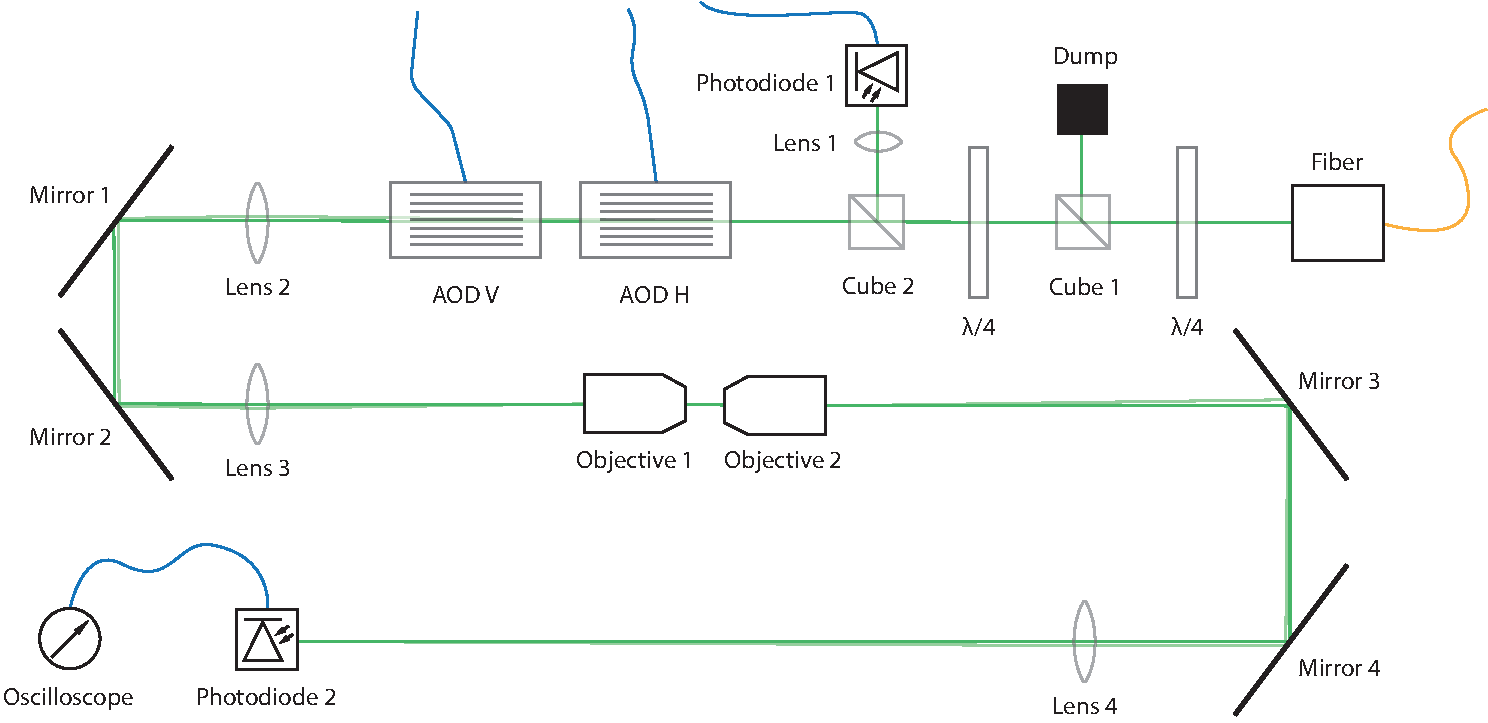
\includegraphics[width=\textwidth]{../media/setup/intensity-distribution.pdf}
  \caption{Experimental setup used to measure the intensity transmission of
    the 2D \gls{aod} in dependence of the configured \gls{dds} signal.
  }\label{fig:intensity_distribution_setup}
\end{figure}

\subsubsection{Digital ramp frequency sweep}

In a first attempt we configure a first \gls{dds} to output a constant
frequency whereas a second \gls{dds} is configured to do a frequency sweep
using the internal digital ramp. After one such sweep the constant frequency
output of the first \gls{dds} is increased and the measurement repeats. The
procedure is repeated until the first \gls{dds} covered the same frequency
range as the second \gls{dds}.
\begin{figure}[htb]
  \centering
  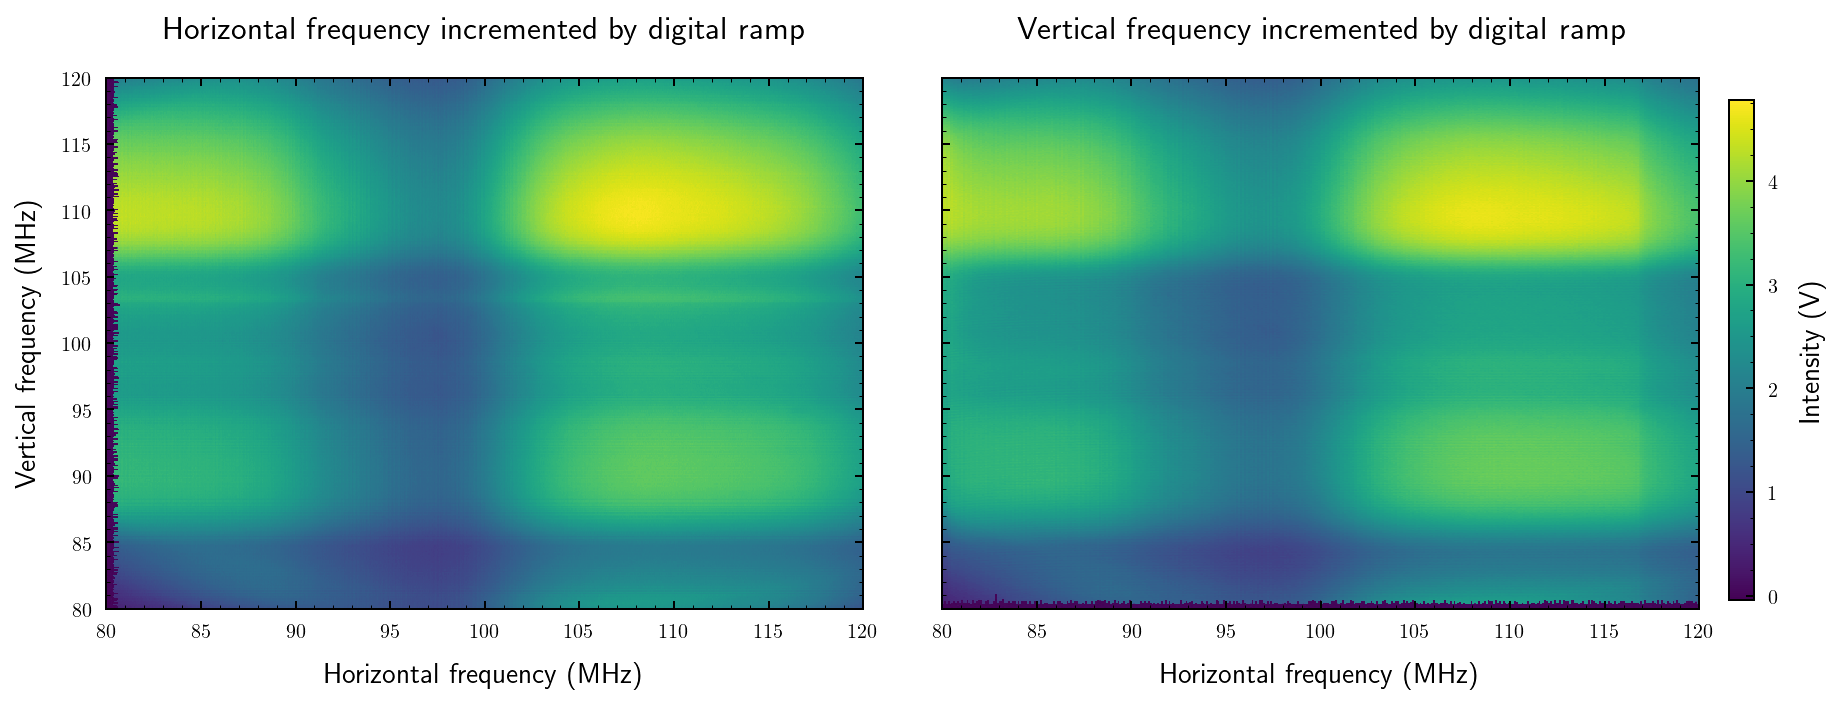
\includegraphics[width=\textwidth]
  {../figure/intensity/distribution/paired-frequency.png}
  \caption{Intensity measured as voltage at the photodiode in dependence of
    the horizontal and vertical applied frequency signal to the \gls{aod}. The
    left map is obtained by enabling the digital ramp on the horizontal
    \gls{dds} whereas the vertical \gls{dds} is configured to output a
    constant frequency which is manually increased after each measurement.
    On the right-hand side map the roles are exchanged.
  }\label{fig:intensity_distribution_frequency}
\end{figure}
In \Cref{fig:intensity_distribution_frequency} we present the intensity
measured at the second photodiode in the setup shown in
\Cref{fig:intensity_distribution_setup}. On the left-hand map the first
\gls{dds} is the \gls{dds} responsible for translations in vertical direction
whereas the second \gls{dds} is responsible for translations in horizontal
direction. The frequency sweep performed by the digital ramp is more dense
compared to the frequency sweep performed by manual increments in our
configuration as the manual increments require driver calls whereas the
digital ramp increments are performed internal of the \gls{dds}.
\begin{figure}[htb]
  \centering
  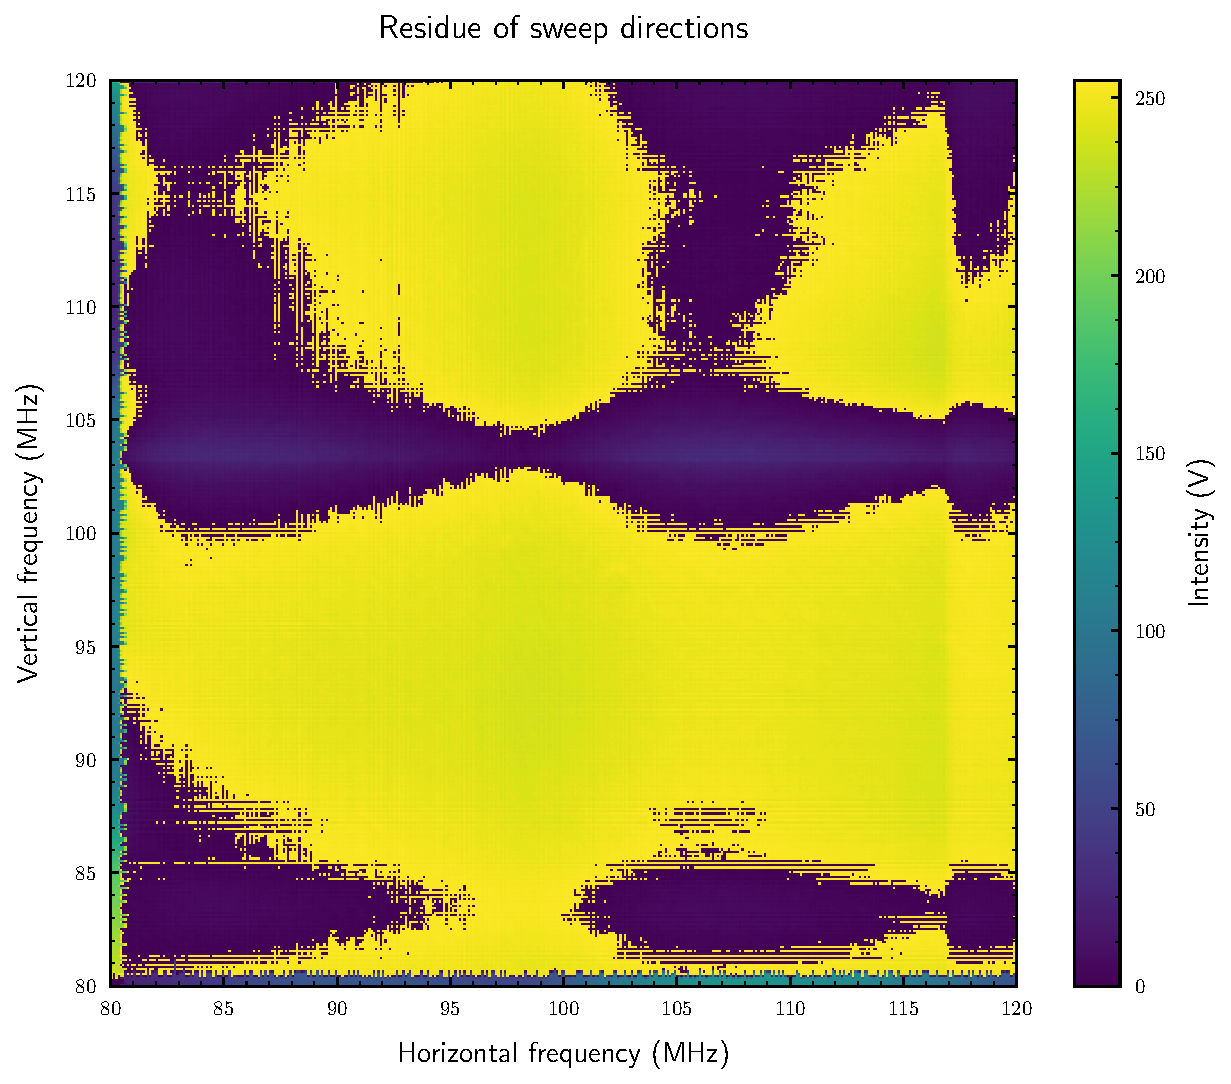
\includegraphics[width=.7\textwidth]
  {../figure/intensity/distribution/paired-frequency-residue.pdf}
  \caption{Absolute difference between the 2D intensity distribution
    performed with the digital ramp configured set to different axes.
  }\label{fig:intensity_distribution_frequency_residue}
\end{figure}
As the differences in \Cref{fig:intensity_distribution_frequency} are of only
subtile nature we additionally reveal the absolute difference between both
maps in \Cref{fig:intensity_distribution_frequency_residue}. We observe
nearly a binary map of dark purple and yellow areas whereas the dark area can
be intepreted as small and the yellow area as large difference. The binary
nature of the absolute difference could be interpreted as a fixed offset
in the power level between the \gls{h} and \gls{v} \gls{rf} signal supplied to
the \gls{aod}s. In areas of small intensity difference (purple) the ouptut
level may be sufficient to saturate the acousto-optics. However we must admit
that these are simply suggestions and need further evidence.

\subsubsection{Constant sampled frequencies}

In \cref{subsec:electronic_amplitude_frequency_response} we did not find
differences in the amplitude frequency response of the amplified \gls{rf}
signal between frequency increments performed by the internal digital ramp of
the \gls{dds} and frequency increments performed by manually updating the
output frequency through the driver. Yet, it remains open if differences
arise in the transmission frequency response of the \gls{aod} as the \gls{aod}
is not a purely electronic device.
\begin{figure}[ht]
  \centering
  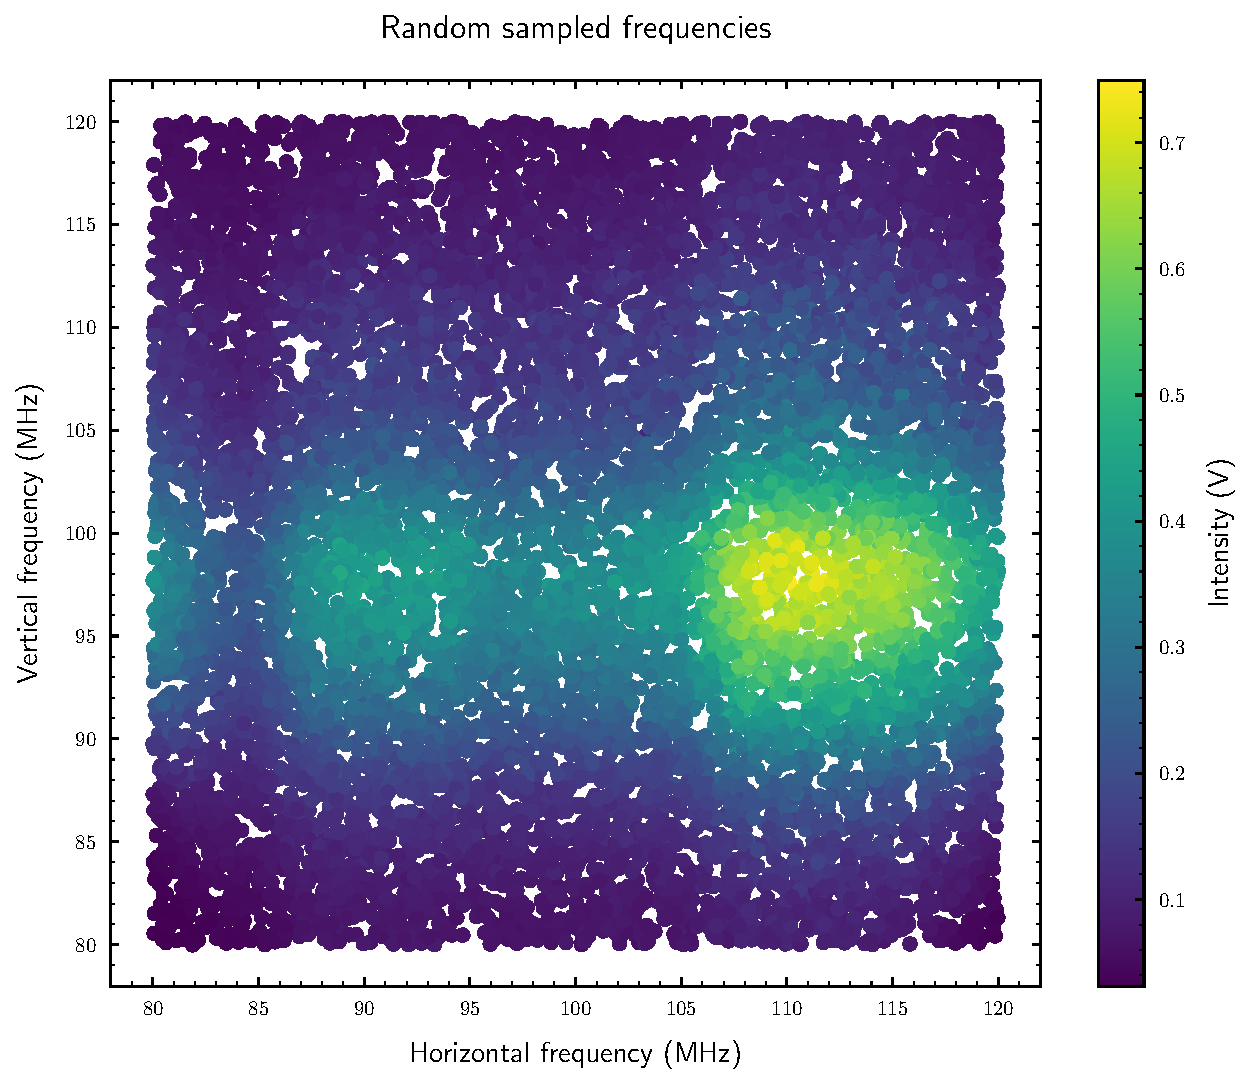
\includegraphics[width=.7\textwidth]
  {../figure/intensity/distribution/sample-frequency.pdf}
  \caption{Intensity measured as voltage at the photodiode in dependence of
    the horizontal and vertical applied frequency signal to the \gls{aod}.
    Frequency pairs are sampled over a uniform distribution and then passed
    as constant output frequency paramter to the \gls{dds}.
  }\label{fig:intensity_distribution_frequency_sampled}
\end{figure}
To partly answer this question we sampled random frequency pairs over a
two dimensional uniform distribution and passed them as constant frequency
parameter to the respective \gls{dds} through the driver interface. The
yielded intensity distribution is visualized in
\Cref{fig:intensity_distribution_frequency_sampled}. We note that in
comparison to \Cref{fig:intensity_distribution_frequency} the intensity
differences are more concentrated around the vertical axis. We believe that
acousto-optics possess a non-instantaneous frequency response characteristic
that requires further investigation.

\subsubsection{Different radio frequency signal source}

In the previous two sections we found that the \gls{aod}s are quite sensible
to the method used to perform frequency increments in a frequency sweep. In
order to further investigate this phenomena we decided to replace one
\gls{dds} with a high-quality signal generator while the other \gls{dds} was
configured to output a constant \SI{100}{\mega\hertz} signal. The output
level of the signal generator was configured to match the output level of
the \gls{dds} and amplified using the usual power amplifier.
\Cref{fig:intensity_distribution_signal_sources} discloses the different
intensity transmission registered by the photodiode for a frequency sweep
performed by the \gls{dds} through the digital ramp and by the signal
generator. In comparison to the \gls{dds} the signal generator does not
support continous frequency changes as we can see from the intensity drops
between the frequency increments of the signal generator trace.
\begin{figure}[htb]
  \centering
  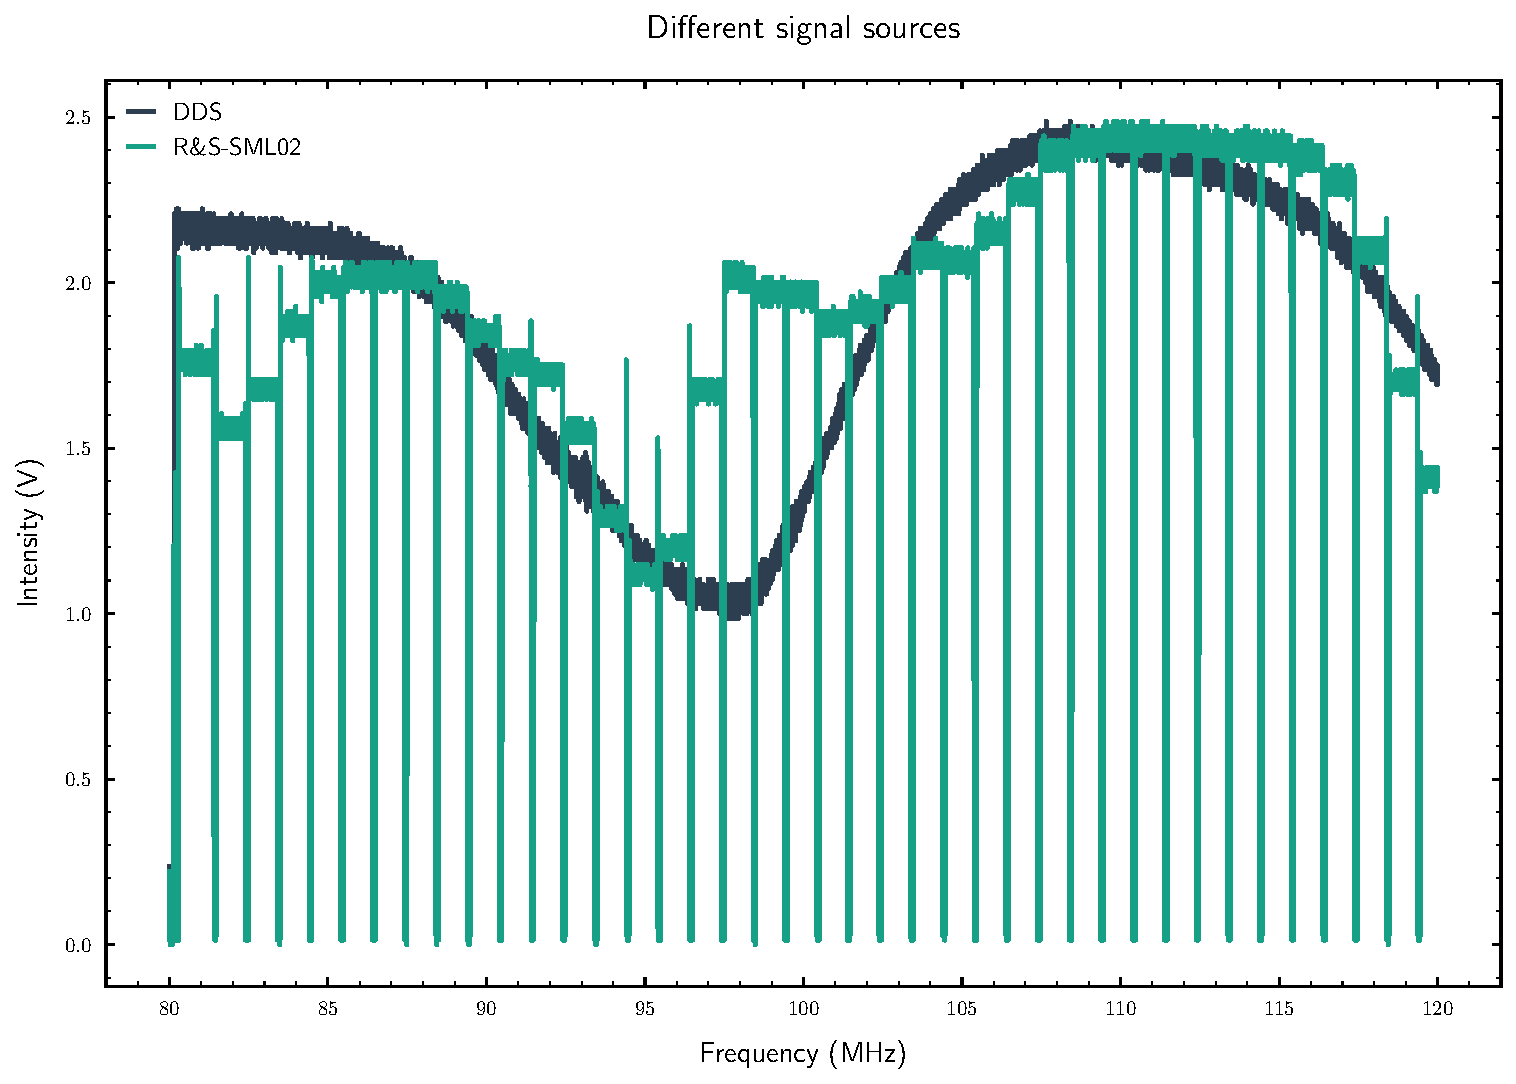
\includegraphics[width=.9\textwidth]{../figure/intensity/distribution/signal-sources.pdf}
  \caption{Intensity measured as voltage at the photodiode with one \gls{aod}
    at constant center frequency supplied by a \gls{dds} and the other
    \gls{aod} performing a linear frequency sweep with the \gls{dds} and a
    high-quality signal generator.
  }\label{fig:intensity_distribution_signal_sources}
\end{figure}
Further ignoring these intensity drops we observe that the global response
characteristics differ in particular at the begin of the frequency sweep and
at the center. As the power amplifier remains unchanged through the
measurements and the output voltage of the signal sources are independent of
frequency, we are only left with two explainations. For one the power supplied
to the \gls{aod} could differ as we did not meausre the current response. On
the other the frequency drops in between frequency increments of the signal
generator could cause the observed characteristis. The later hyphothesis would
also confirm the result of the previous section in which we found a different
transmission characteristic for differen frequency sampling strategies.

\subsubsection{Summary}

In summary we found that the intensity transmission of the \gls{aod} show a
highly non-linear dependency in the applied power and the method used for
frequency sampling. It will continue to be interesting to explore the
intensity transmission subject to the effective power of the \gls{rf} signal
applied to the \gls{aod}. So far we only know that the voltage of the \gls{rf}
signal of the \gls{dds} is constant over our frequency range of
\SI{80}{\mega\hertz} to \SI{120}{\mega\hertz}, however we cannot make any
statements with respect to the current characteristics. All in all there are
too many factors to consider to describe with a simple analytical model and we
will further try to work with a model-free optimization procedure in the next
chapter in order to minimize the intensity transmission variance and produce
a constant laser intensity in the atom plane.
